% HIKET figure storyboard (working draft) -- LaTeX + TikZ.
% Compile: pdflatex FIGURE_STORYBOARD_DRAFT.tex  (run from manuscript/).
\documentclass[10pt]{article}
\usepackage[utf8]{inputenc}
\usepackage[T1]{fontenc}
\usepackage[margin=2cm]{geometry}
\usepackage{graphicx}
\usepackage{amsmath}
\usepackage{xcolor}
\usepackage{float}
\usepackage[hidelinks]{hyperref}
\usepackage{tikz}
\usetikzlibrary{positioning, arrows.meta, calc, fit, backgrounds}

\newcommand{\sinit}{\sigma_{\mathrm{init}}}
\newcommand{\sinput}{\sigma_{\mathrm{input}}}
\newcommand{\wh}[1]{\textbf{What:}~#1}
\newcommand{\ft}[1]{\textbf{Fits:}~#1}
% figure paths (relative to manuscript/)
\newcommand{\mm}{../Calibration_real_data_transient/diagnostics/multimodel}
\newcommand{\dg}{../Calibration_real_data_transient/diagnostics}
\newcommand{\rep}{../Reporting/NextgenC_report}
\newcommand{\CID}{20260710_104903_20260710_104904_20260710_104904_20260710_104902_20260710_104902_20260710_102431}

\title{\vspace{-1.5cm}HIKET --- figure storyboard (working draft)}
\author{}
\date{Figures in narrative order (Schimel OCAR). Flux-bounded 20260710 run. Compiled \today.}

\begin{document}
\maketitle
\vspace{-0.8cm}

\noindent\emph{Protagonist} = the initialization problem. \emph{Trickster} = $\sinput$ (input/history
uncertainty). Very short notes per figure. All F1--F14 and the robustness set (S1--S7) are built.

% =====================================================================
\section*{Storyline schema (main arc + side arcs)}

\begin{center}
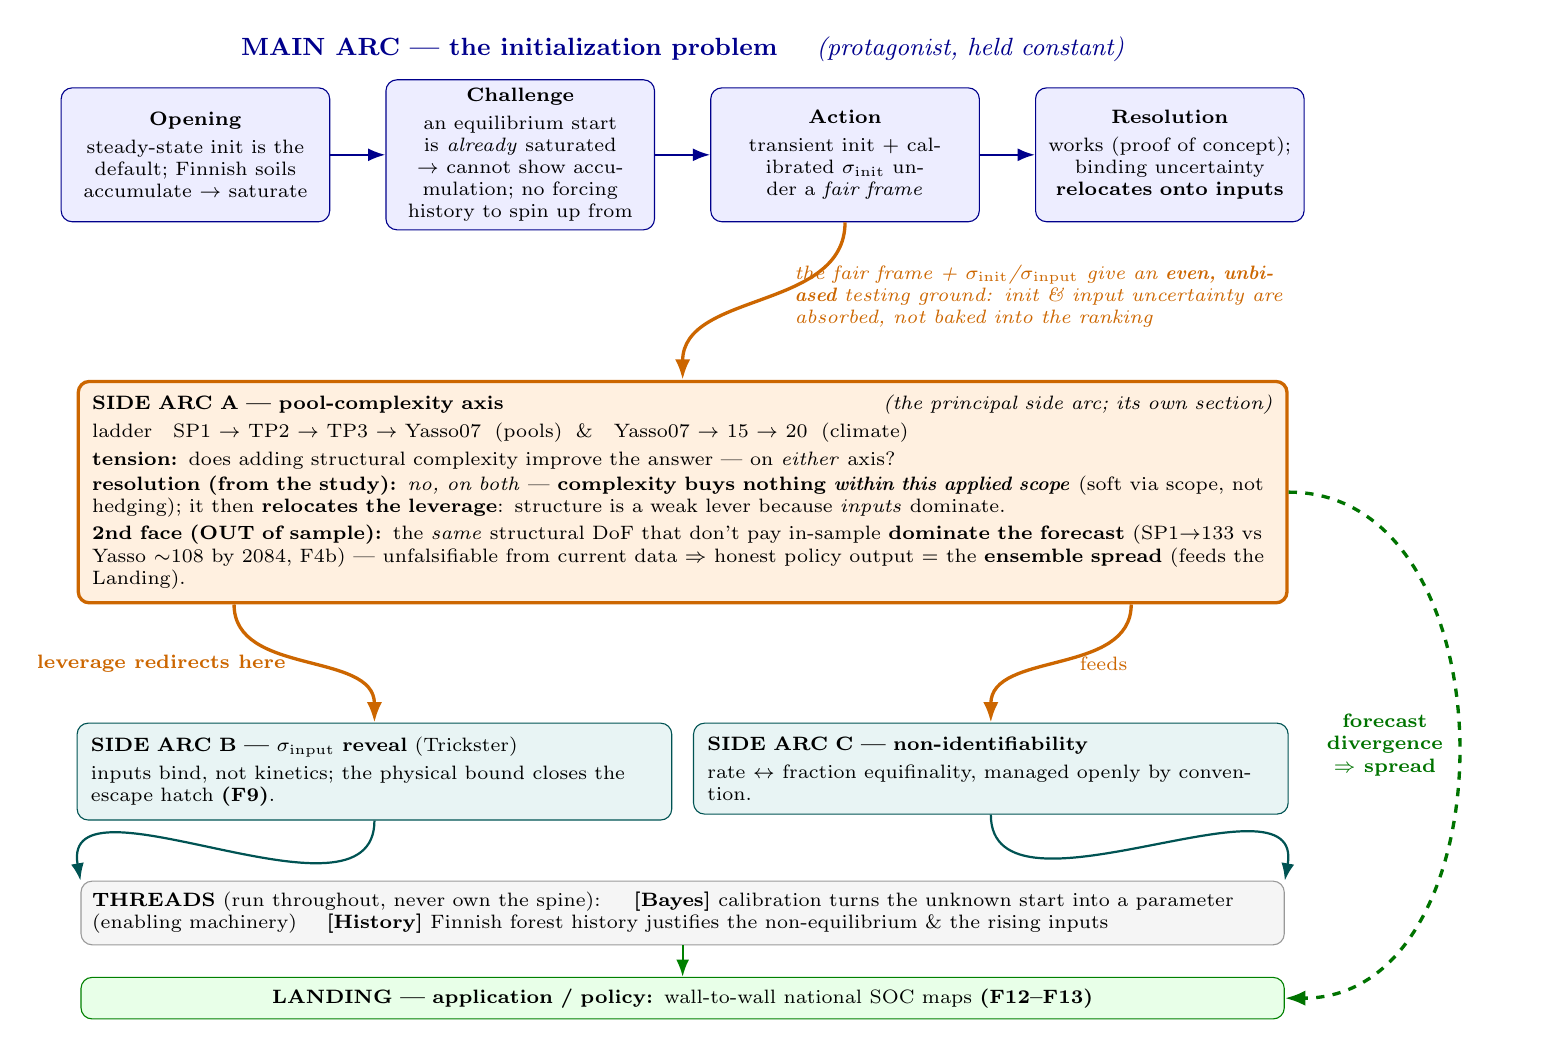
\begin{tikzpicture}[
  font=\scriptsize,
  ocar/.style={rectangle, rounded corners, draw=blue!55!black, fill=blue!7, align=center,
               text width=32mm, minimum height=17mm, inner sep=3pt},
  arca/.style={rectangle, rounded corners, draw=orange!80!black, fill=orange!12, very thick,
               align=left, text width=150mm, inner sep=5pt},
  arcbc/.style={rectangle, rounded corners, draw=teal!65!black, fill=teal!9, align=left,
                text width=72mm, inner sep=5pt},
  land/.style={rectangle, rounded corners, draw=green!50!black, fill=green!9, align=center,
               text width=150mm, inner sep=4pt},
  thread/.style={rectangle, rounded corners, draw=black!40, fill=black!4, align=left,
                 text width=150mm, inner sep=4pt},
  fl/.style={-{Latex[length=2.2mm]}, thick, blue!55!black},
  flo/.style={-{Latex[length=2.6mm]}, very thick, orange!80!black},
  lbl/.style={align=left, font=\scriptsize\itshape, text width=62mm},
]
% --- OCAR row ---
\node[ocar] (O) {\textbf{Opening}\\[2pt] steady-state init is the default; Finnish soils accumulate $\to$ saturate};
\node[ocar, right=7mm of O] (C) {\textbf{Challenge}\\[2pt] an equilibrium start is \emph{already} saturated $\to$ cannot show accumulation; no forcing history to spin up from};
\node[ocar, right=7mm of C] (A) {\textbf{Action}\\[2pt] transient init + calibrated $\sinit$ under a \emph{fair frame}};
\node[ocar, right=7mm of A] (R) {\textbf{Resolution}\\[2pt] works (proof of concept); binding uncertainty \textbf{relocates onto inputs}};
\draw[fl] (O)--(C); \draw[fl] (C)--(A); \draw[fl] (A)--(R);
% banner
\node[above=2mm of $(O.north)!0.5!(R.north)$, font=\small\bfseries, blue!55!black]
  {MAIN ARC --- the initialization problem \quad\mdseries\itshape(protagonist, held constant)};
% --- Side Arc A ---
\coordinate (mid) at ($(O.south)!0.5!(R.south)$);
\node[arca, below=20mm of mid] (SA)
  {\textbf{SIDE ARC A --- pool-complexity axis}\hfill\textit{(the principal side arc; its own section)}\\[2pt]
   ladder \; SP1 $\to$ TP2 $\to$ TP3 $\to$ Yasso07 \;(pools)\; \& \; Yasso07 $\to$ 15 $\to$ 20 \;(climate)\\[2pt]
   \textbf{tension:} does adding structural complexity improve the answer --- on \emph{either} axis?\\[1pt]
   \textbf{resolution (from the study):} \emph{no, on both} --- \textbf{complexity buys nothing
   \emph{within this applied scope}} (soft via scope, not hedging); it then \textbf{relocates the
   leverage}: structure is a weak lever because \emph{inputs} dominate.\\[2pt]
   \textbf{2nd face (OUT of sample):} the \emph{same} structural DoF that don't pay in-sample
   \textbf{dominate the forecast} (SP1$\to$133 vs Yasso $\sim$108 by 2084, F4b) --- unfalsifiable from
   current data $\Rightarrow$ honest policy output = the \textbf{ensemble spread} (feeds the Landing).};
\draw[flo] (A.south) to[out=-90,in=90]
  node[lbl, right=1mm, pos=0.45]{the fair frame + $\sinit$/$\sinput$ give an \textbf{even, unbiased} testing ground: init \& input uncertainty are absorbed, not baked into the ranking} (SA.north);
% --- Side arcs B / C ---
\node[arcbc, below=15mm of SA.south west, anchor=north west] (SB)
  {\textbf{SIDE ARC B --- $\sinput$ reveal} (Trickster)\\[2pt]
   inputs bind, not kinetics; the physical bound closes the escape hatch \textbf{(F9)}.};
\node[arcbc, below=15mm of SA.south east, anchor=north east] (SC)
  {\textbf{SIDE ARC C --- non-identifiability}\\[2pt]
   rate $\leftrightarrow$ fraction equifinality, managed openly by convention.};
\draw[flo] (SA.south west)++(20mm,0) coordinate(sal) (sal) to[out=-90,in=90]
  node[font=\scriptsize\bfseries, orange!80!black, left=1mm, pos=0.5]{leverage redirects here} (SB.north);
\draw[flo] (SA.south east)++(-20mm,0) coordinate(sar) (sar) to[out=-90,in=90]
  node[font=\scriptsize, right=1mm, pos=0.5]{feeds} (SC.north);
% --- threads + landing ---
\node[thread, below=8mm of $(SB.south east)!0.5!(SC.south west)$, anchor=north] (TH)
  {\textbf{THREADS} (run throughout, never own the spine): \quad
   \textbf{[Bayes]} calibration turns the unknown start into a parameter (enabling machinery) \quad
   \textbf{[History]} Finnish forest history justifies the non-equilibrium \& the rising inputs};
\node[land, below=4mm of TH] (LA)
  {\textbf{LANDING --- application / policy:} wall-to-wall national SOC maps \textbf{(F12--F13)}};
\draw[fl, green!50!black] (TH)--(LA);
\draw[fl, teal!65!black] (SB.south) to[out=-90,in=100] (TH.north west);
\draw[fl, teal!65!black] (SC.south) to[out=-90,in=80] (TH.north east);
% Side Arc A's 2nd (out-of-sample) face feeds the policy landing directly
\draw[flo, dashed, green!45!black] (SA.east) to[out=0,in=0,looseness=1.15]
  node[font=\scriptsize\bfseries, green!45!black, left=0.5mm, pos=0.5, align=center]
  {forecast\\divergence\\$\Rightarrow$ spread} (LA.east);
\end{tikzpicture}
\end{center}

\noindent Vertical link: the main arc's machinery (transient init + the two $\sigma$'s) is what makes
SIDE ARC~A a \emph{fair} test --- models compete on structure, not on who guessed inputs / initial state best.

% =====================================================================
\section*{Opening / Challenge --- the phenomenon and the trap}

\paragraph{F1 $\cdot$ The inputs (redesigned --- inputs-first).}
\begin{center}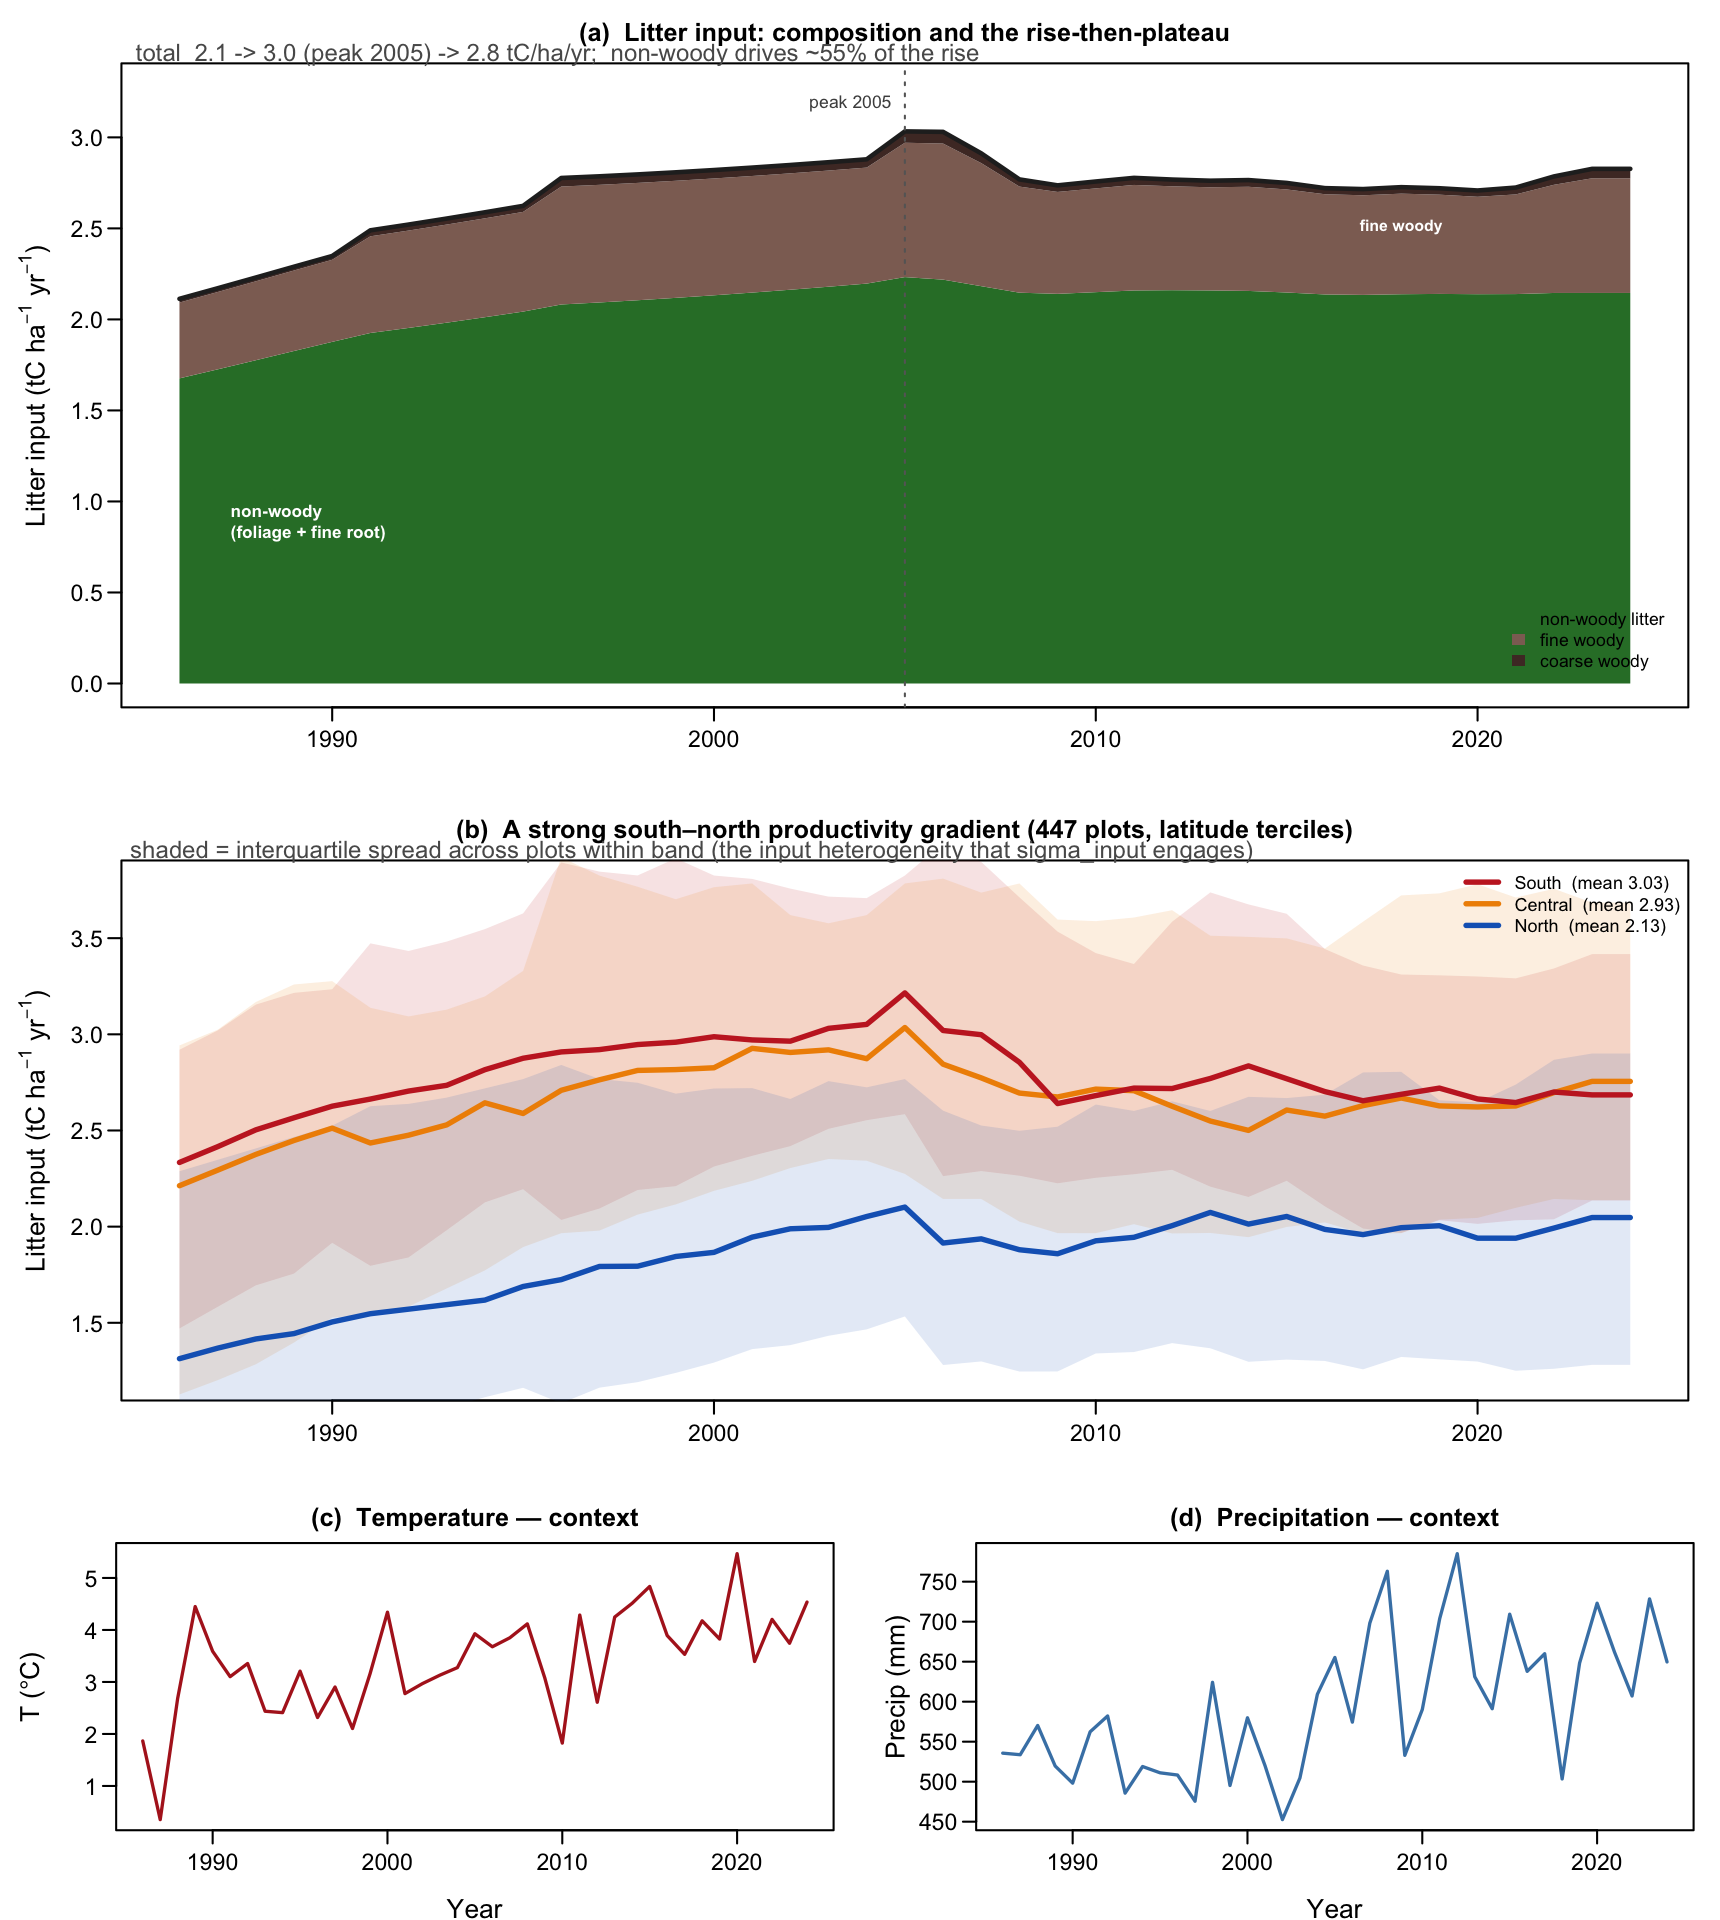
\includegraphics[width=0.86\linewidth]{figures/F1_inputs.png}\end{center}
\wh{three views of the litter input, with climate demoted to a supporting strip. \textbf{(a)} composition
over time --- stacked non-woody / fine-woody / coarse-woody: total rises $2.1\!\to\!3.0$ (peak 2005) then
plateaus $\sim$2.8; \emph{non-woody foliage/fine-root litter drives $\sim$55\% of the rise}. \textbf{(b)}
a strong south--north gradient (447 plots, latitude terciles: mean 3.0 / 2.9 / 2.1 tC/ha/yr) with the
wide within-band plot spread shaded. \textbf{(c,d)} $T$ and $P$ --- interannual swings, no accumulation
trend --- shown small, as context only.}
\ft{makes the opening about \textbf{inputs}, not climate. (a) the smooth rise-then-plateau $\Rightarrow$
accumulation is input/history-driven (motivates transient init + the [History] thread); (b) inputs vary
enormously in \emph{space} --- the heterogeneity that $\sinput$ and site productivity (F11) engage, and
the spatial face of the SOC maps (F12); (c,d) climate is jagged/trendless $\Rightarrow$ any interannual
SOC wiggle is climate, not accumulation. Foreshadows the $\sinput$ reveal. \emph{Script:}
\texttt{figures/build\_F1\_inputs.R} (Yasso20 bundle --- the size-class split lives only in the Yasso inputs).}

\paragraph{F2 $\cdot$ Uncalibrated baseline under-predicts (redesigned --- general, cross-plot mean).}
\begin{center}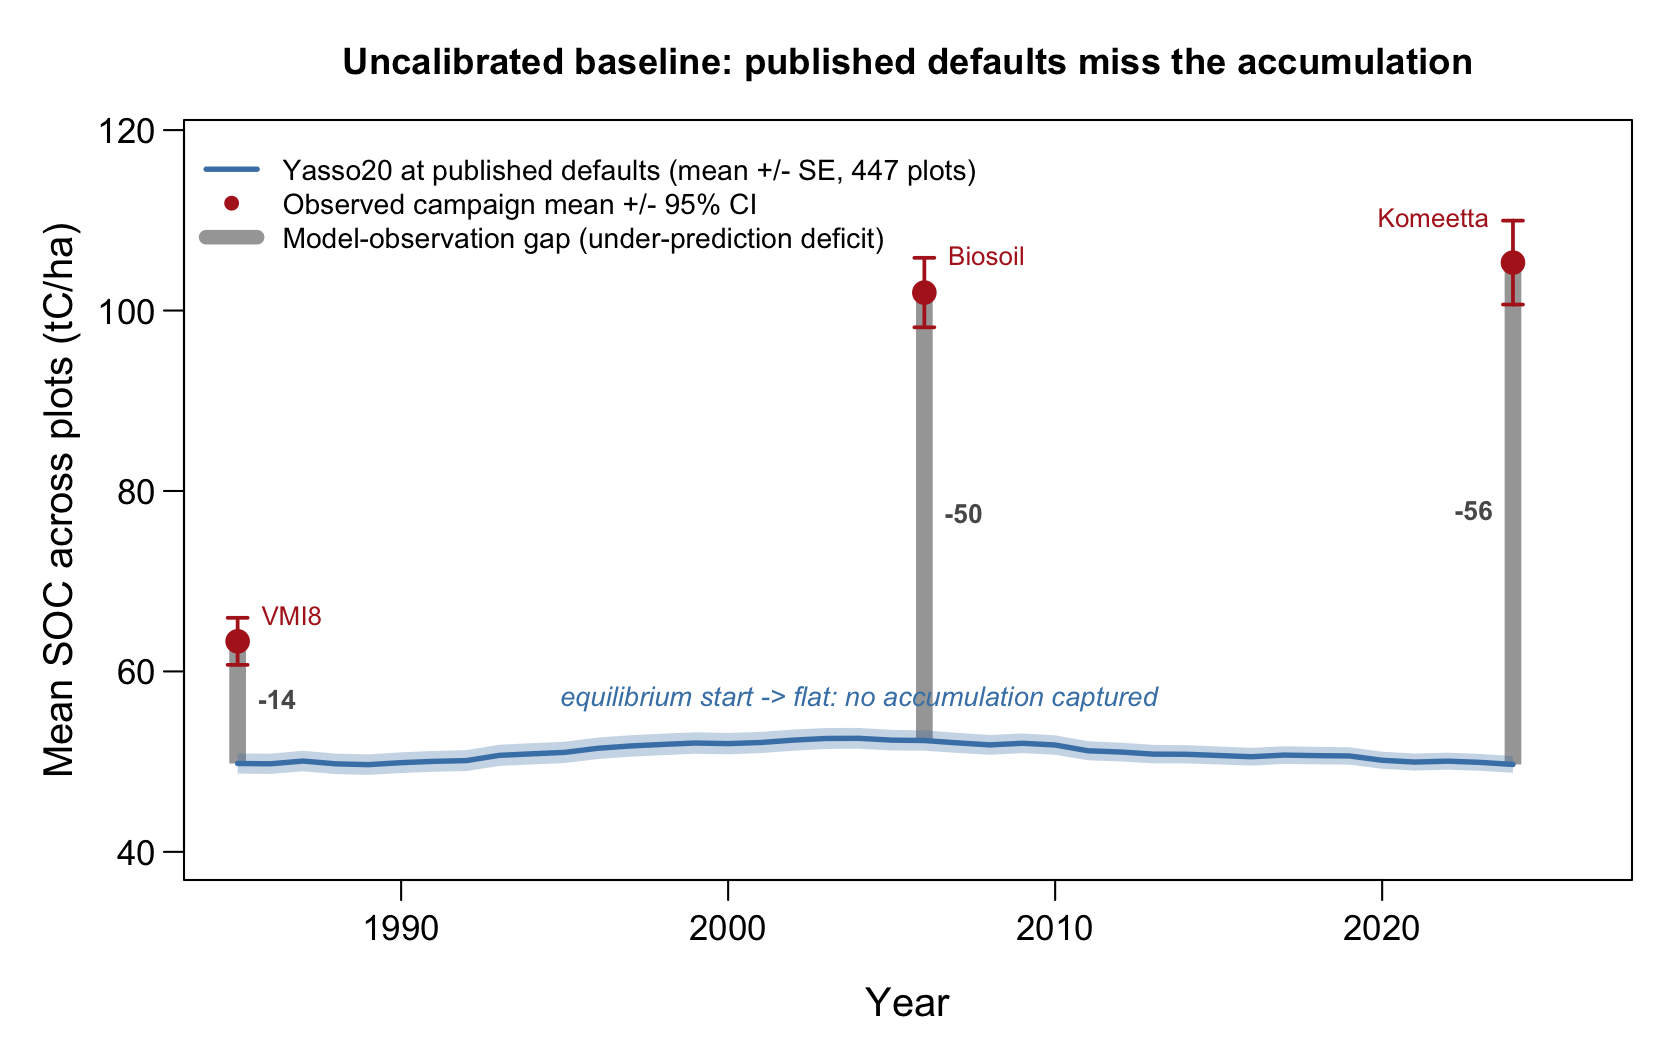
\includegraphics[width=0.82\linewidth]{figures/F2_baseline.png}\end{center}
\wh{Yasso20 forward at published defaults ($\sinput=1$) with the conventional equilibrium start,
\emph{averaged over all 447 plots} (like F3, not 4 example plots). The baseline sits \textbf{flat at
$\sim$50 tC/ha}; the observed campaign means climb $63\to102\to105$ --- a widening deficit of
$-14/-50/-56$ tC/ha.}
\ft{two failures in one glance. (1) \textbf{Flat} --- an equilibrium start is \emph{already} at its
steady state, so it cannot accumulate: the OCAR \emph{Challenge} made visual (motivates the transient-init
protagonist). (2) \textbf{Low} --- boreal-blind published defaults sit far below the stocks (the Mentor
beat): the lineage is real but the \emph{start}, not the soil, is wrong. \emph{Script:}
\texttt{figures/build\_F2\_baseline.R} (baseline predictions + observed campaign means; defaults are
calibration-independent, so no RUN\_ID coupling).}

% =====================================================================
\section*{Action / Results --- the protagonist pays off (H1)}

\paragraph{F3 $\cdot$ Mean-SOC trajectories, six models (headline; rebuilt, uniform palette).}
\begin{center}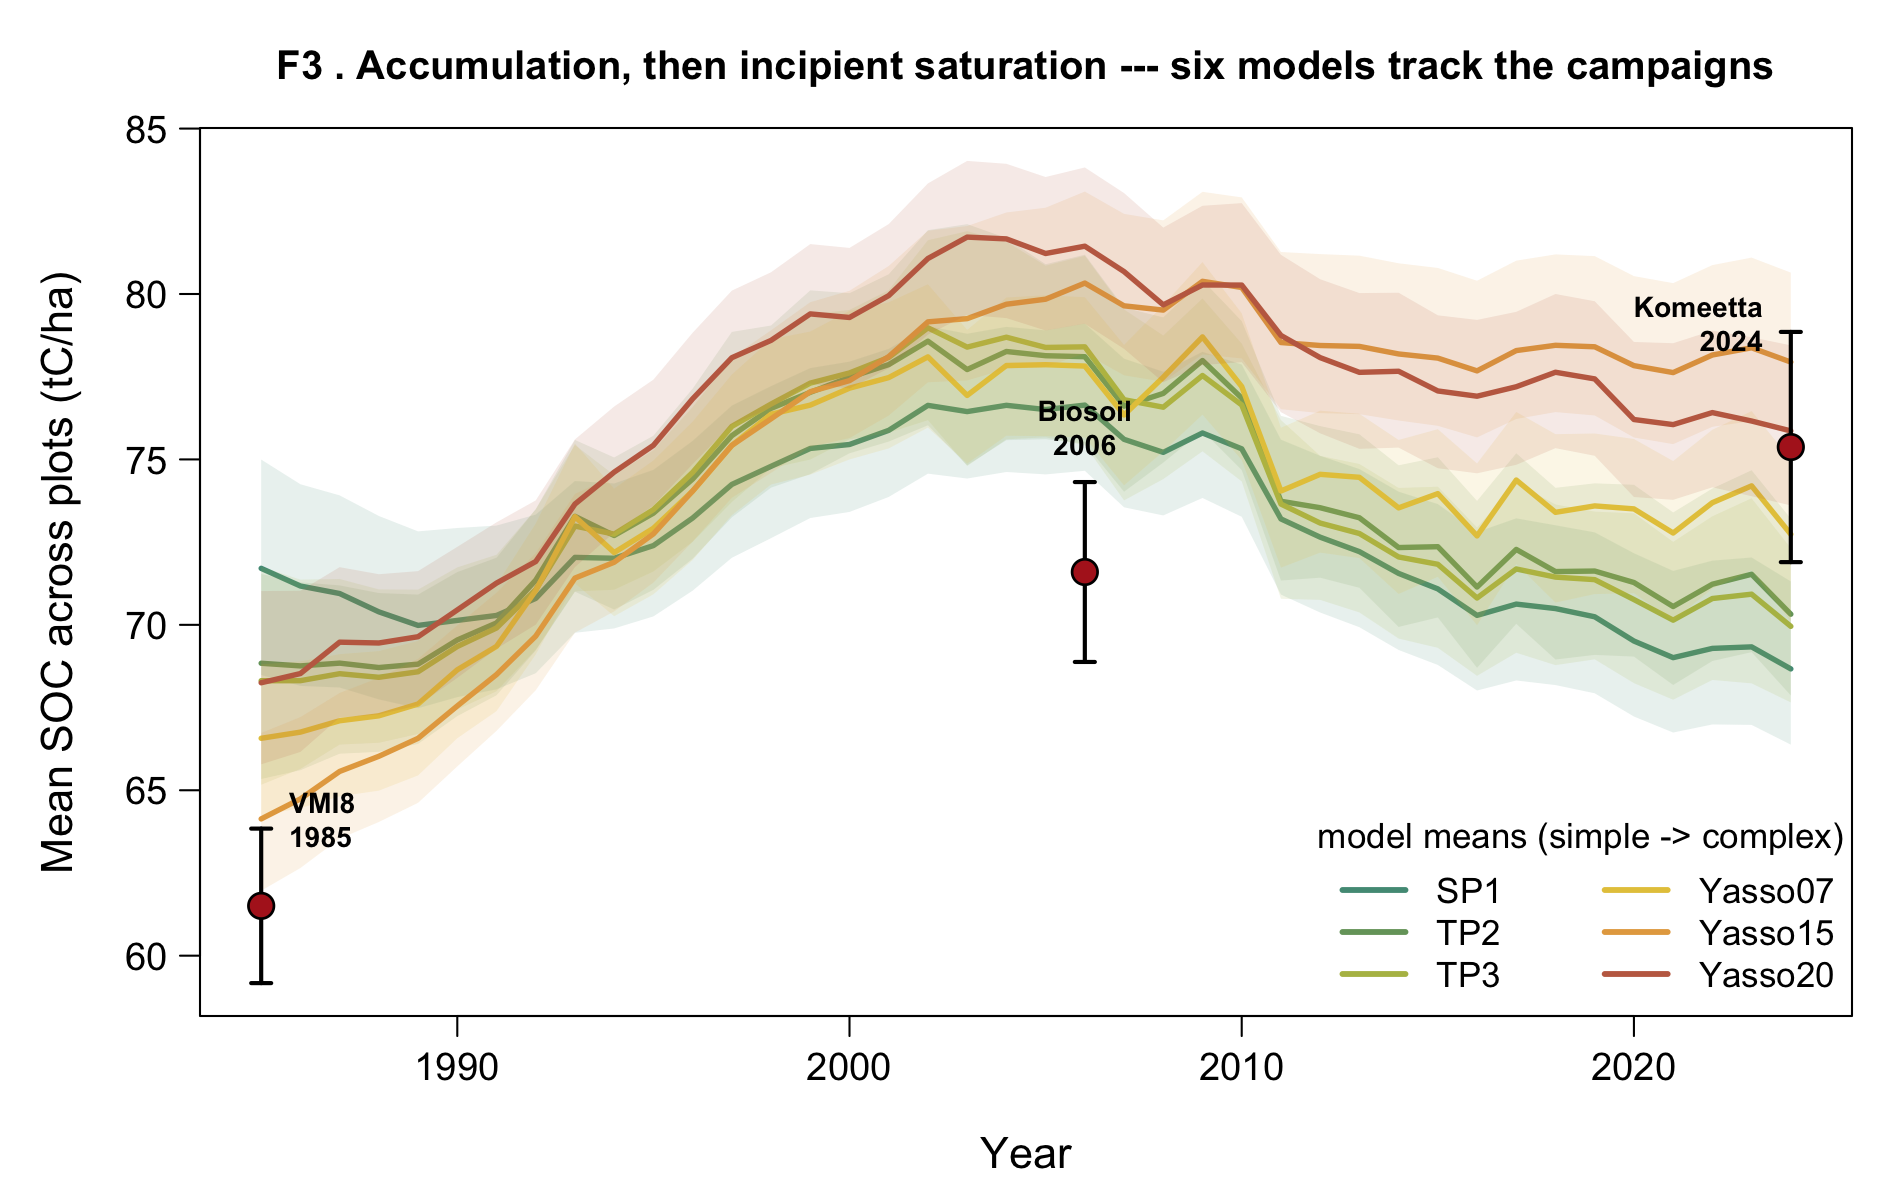
\includegraphics[width=0.88\linewidth]{figures/F3_mean_soc.png}\end{center}
\wh{cross-plot mean SOC $1985\to2024$; all six rise then bend toward saturation, tracking the Biosoil/Komeetta
campaign means. Shared model palette (green simple trio $\to$ warm Yasso trio). \emph{Script:} \texttt{build\_F3\_mean\_soc.R}.}
\ft{\textbf{H1} --- transient init reproduces accumulation-then-saturation, the shape an equilibrium start forecloses. The central proof of concept.}

\paragraph{F4 $\cdot$ The initialization problem (redesigned --- 2-panel: past spin-up + future forecast).}
\begin{center}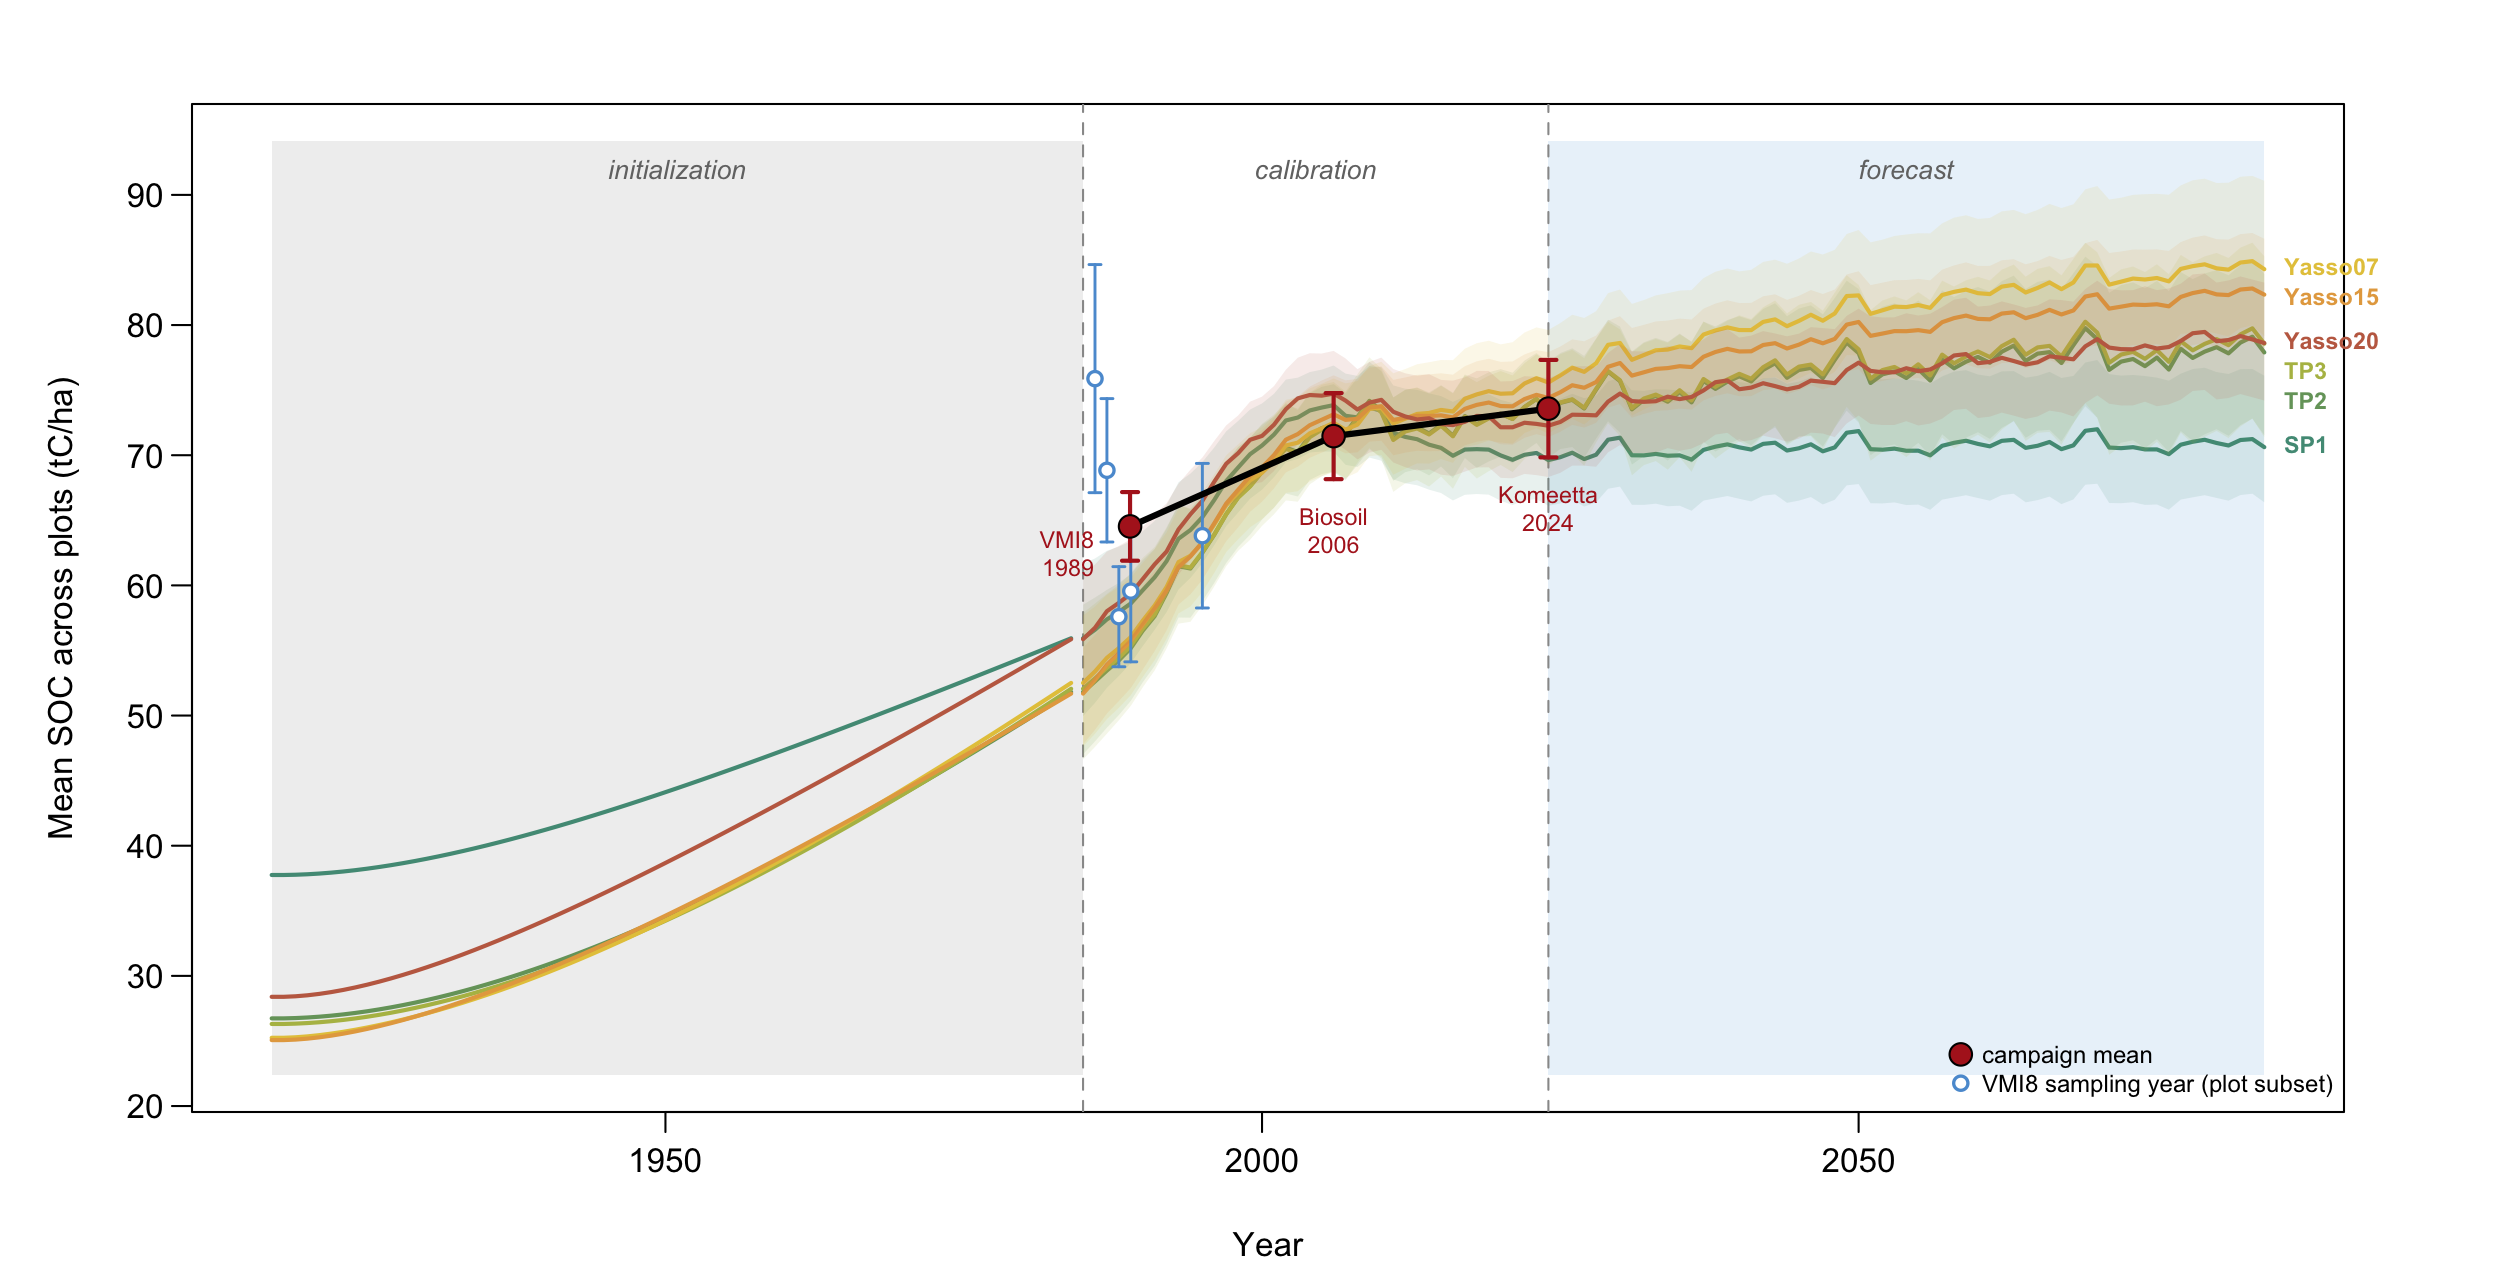
\includegraphics[width=0.98\linewidth]{figures/F4_initialization.png}\end{center}
\wh{six model means, same colour code, posterior ribbons in the observed/forecast windows. \textbf{(a)}
the \emph{full} trajectory including the modelled transient-init spin-up $1917\to1985$ (median line;
constant climate + linearly ramped litter from a below-equilibrium 1917 anchor, level pinned to the
calibrated 1985 stock) + observed window on the observed path ($63\to102\to105$): all models reach
$\sim$90 in 1985 --- \textbf{$+26$ tC/ha above the observed start} --- and climb only $\sim$$+0.70$
tC/ha/yr through 2006 vs the data's $+1.84$. \textbf{(b)} the \emph{future forecast} $2025\to2084$: models
agree in the calibrated window but \emph{fan out sharply} (SP1 $\to$133 with no saturation; Yasso15/20
plateau $\sim$108).}
\ft{the candid beat of the protagonist's payoff. (a) makes the transient-init machinery visible: each
model recovers from a below-equilibrium 1917 anchor --- \emph{but the structures disagree about how much}
(simple models recover strongly from $\sim$70--80; Yasso15/20 start near-full $\sim$93--96), and all
converge $\sim$26 tC/ha above the observed 1985 start (the open [[transient-phase-open-question]], a live
question not a failure). (b) is the structural-divergence story: equal where calibrated, divergent when
extrapolated. \emph{Secondary:} shape-divergence is expressiveness in the unobserved past/future, not
data-constrained skill (honest lead-in to Side Arc~A). \emph{Reconciliation} of the earlier
cumulative-average-rate figure: appendix ``Reconciling the SOC-change diagnostics.''
\emph{Scripts:} \texttt{build\_F4\_initialization.R} (caches the spin-up reconstruction to
\texttt{F4\_cache.rds}), \texttt{build\_appendix\_delta\_reconciliation.R}. \emph{Palette (2026-07-15):}
continuous \emph{diverging} ramp \texttt{ggthemes::Temperature Diverging} --- the two hue-sides also \textbf{class
the two model families}: green-ish simple trio (SP1/TP2/TP3) vs warm gold$\to$rust Yasso trio (07/15/20), saturated
centre (no washed middle). Applied uniformly across all by-model figures via the shared \texttt{model\_palette.R}.}

\paragraph{T1 $\cdot$ Results at a glance --- the numbers F4 no longer shows (per-model summary table).}
\begin{center}\small% auto-generated by build_T1_model_summary.R -- per-model summary
\begin{tabular}{lccccccc}
\hline
Model & Pools & Free & $R^2$ & $R^2$ & RMSE & Eff.\ flux & $\sigma_{\mathrm{init}}$ \\
 & & params & (cal) & (hold) & (hold) & $\sigma_{\mathrm{inp}}\bar J$ & \\
\hline
SP1 & 1 & 6 & 0.017 & 0.000 & 46 & 4.9 & 0.67 \\
TP2 & 2 & 7 & 0.018 & 0.000 & 47 & 6.4 & 0.40 \\
TP3 & 3 & 9 & 0.019 & 0.000 & 47 & 6.5 & 0.37 \\
Yasso07 & 5 & 20 & 0.028 & 0.002 & 45 & 6.6 & 0.24 \\
Yasso15 & 5 & 26 & 0.031 & 0.004 & 44 & 5.9 & 0.18 \\
Yasso20 & 5 & 26 & 0.023 & 0.001 & 45 & 6.6 & 0.21 \\
\hline
\end{tabular}
\normalsize\end{center}
\wh{one row per model: structural complexity (pools, free params), skill ($R^2$ calibration \& holdout, holdout
RMSE), the inputs story (effective litter flux $\sinput\bar J$, tC\,ha$^{-1}$\,yr$^{-1}$; all now inside the
physical [0.5,\,8.7] envelope), and the initial state ($\sinit<1$). Generated by \texttt{build\_T1\_model\_summary.R}.}
\ft{the whole thesis in eight columns. \textbf{Complexity climbs, skill does not:} pools $1\to5$ / free params
$6\to26$, yet calibration $R^2$ \emph{falls} $0.079\to0.062$ (Yasso20 worst) and holdout $R^2$ stays $\sim$0.02--0.04.
\textbf{Inputs bind:} the two former runaways TP2/TP3 sit highest ($\sim$6.1--6.2) but now physical. \textbf{Below-
equilibrium start:} every $\sinit<1$. Read alongside F4b, the 2084 forecast fans $133\to108$ --- the divergence
skill cannot adjudicate. This is the table the redesigned F4 (trajectories-only) dropped; keep it beside F4.}

% =====================================================================
\section*{Action / Results --- structural skill under the fair frame (H2)}

\paragraph{F6 $\cdot$ Observed vs predicted --- HOLDOUT only, points classed by stand basal area (redesigned).}
\begin{center}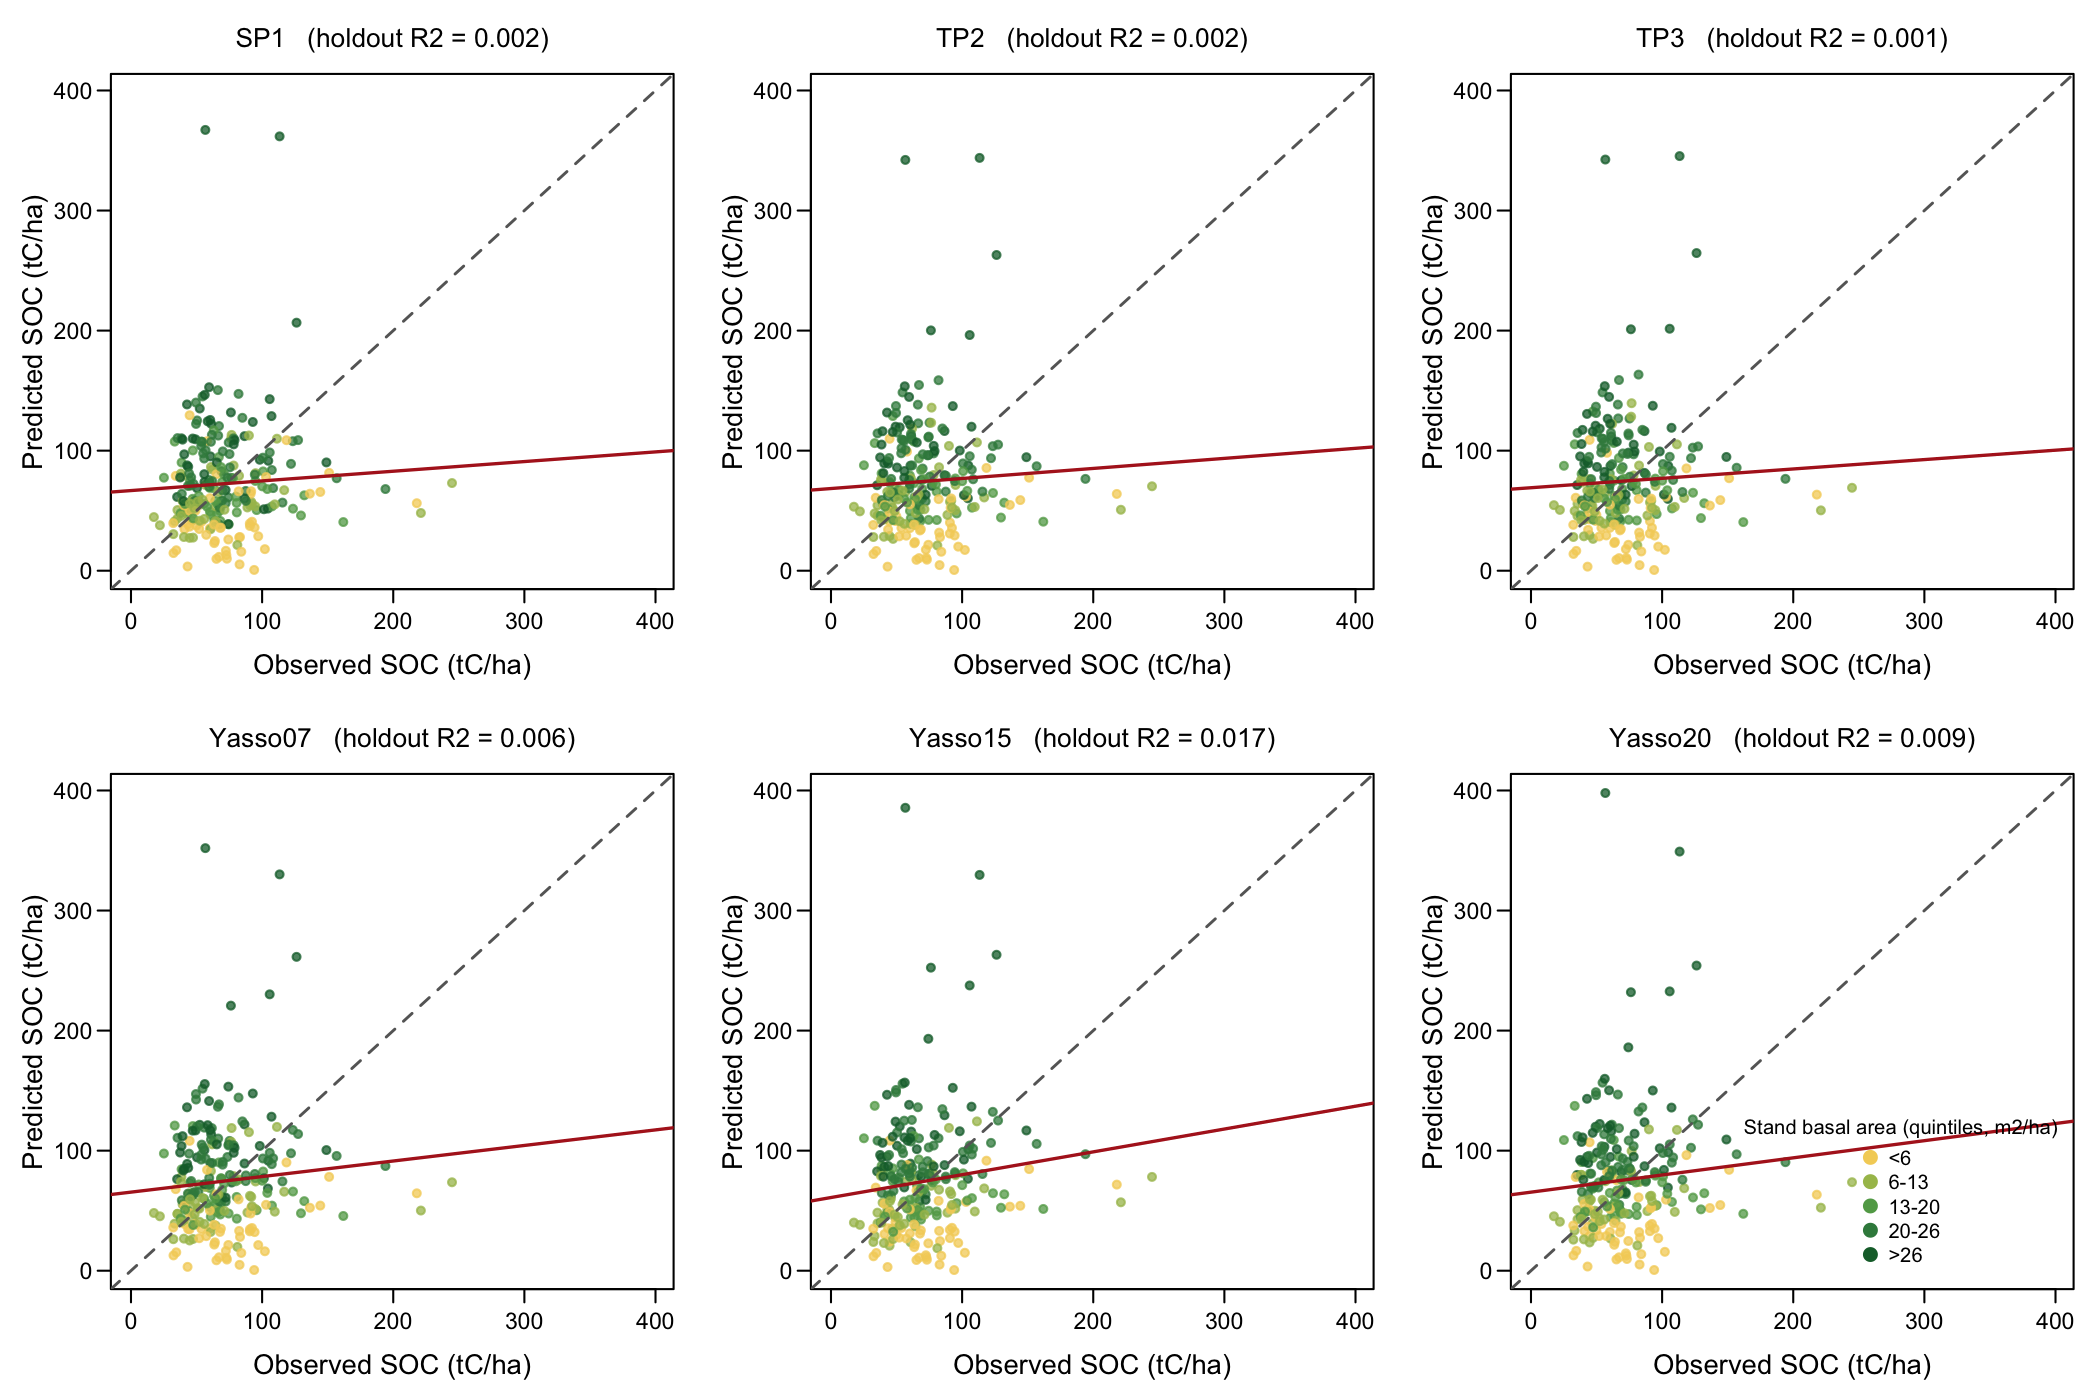
\includegraphics[width=0.98\linewidth]{figures/F6_obs_vs_pred_holdout.png}\end{center}
\wh{plot-level posterior median vs observed SOC on the \textbf{held-out} plots (calibration panel $\to$
supplementary), 2$\times$3 by model; points coloured by \textbf{stand basal-area quintile} (\texttt{Green-Gold}: gold low
$\to$ dark green high). \textbf{Dashed grey = 1:1} (perfect prediction); \textbf{red = linear least-squares
(OLS) fit} = the actual predicted-vs-observed trend --- much flatter than 1:1, i.e.\ the models compress the
range (over-predict low-SOC plots, under-predict high). Holdout $R^2$ per panel (0.015--0.037).}
\ft{\textbf{H2} on the honest set --- skill is uniformly low and the between-model ranking nearly collapses out of
sample (Yasso20 lowest, 0.015; TP3 highest, 0.037). Classing by basal area puts the \#1 residual driver (F11)
\emph{inside} the cloud: the model \emph{predictions} climb with basal area (dark points sit higher) through the
litter inputs, but observed SOC does not track it as tightly --- so the productivity signal lives in the forcing,
not in recoverable skill. Sets up ``inputs are the lever'' (Side Arc~B) and the residual-driver arc (F11).
\emph{Script:} \texttt{build\_F6\_obs\_vs\_pred\_holdout.R}. \emph{Bounding inputs cost skill \emph{only} for
TP2/TP3} (before/after: \S sigma-input appendix).}

% =====================================================================
\section*{SIDE ARC A --- Pool-complexity axis: does complexity improve the answer?}
\textit{The principal side narrative --- its own section. It carries a self-contained tension and
resolution, and it serves the spine rather than competing with it.}

\paragraph{Why the test is fair (link to the main arc).}
The comparison only means anything if the models are not secretly competing on who guessed the inputs
or the initial state best. Transient init + the two auxiliary $\sigma$'s provide exactly that even
ground: $\sinit$ absorbs the unknown historical start, $\sinput$ the litter-input uncertainty, both
homogeneously and with uncertainty propagated. So the six structures ``battle'' on an unbiased field
--- the ranking reflects \textbf{structure}, not input/init luck.

\paragraph{The ladder --- each rung a probe.}
\textbf{SP1 (1 pool)} the Occam floor: the minimal model already reproduces
accumulation$\to$saturation and is competitive; the study's only identified rate --- proof the
\emph{start}, not the structure, is the hero. \;
\textbf{TP2 (2 pools)} the fast/slow split made visible: the pool-memory mechanism that justifies
transient init; textbook-clean control. \;
\textbf{TP3 (3-pool cascade)} the cautionary rung: the extra pool buys non-identifiability + input
compensation + oscillation, not skill --- the clearest escape-hatch victim. \;
\textbf{$\to$ Yasso07/15/20} rates fixed; the operational destination (pools \emph{and} the
climate-integration sub-axis).

\paragraph{The tension.} Does climbing structural complexity improve the answer --- on \emph{either}
axis (pools SP1$\to$Yasso07, climate Yasso07$\to$15$\to$20)?

\paragraph{The resolution --- complexity buys nothing \emph{within this scope} (soft but firm).}
\emph{No, on both axes.} Skill does not climb either ladder: calibration $R^2$ stays 0.047--0.077
(holdout 0.015--0.037), the pool-axis OLS slope is \emph{negative}, and the \emph{most} complex model,
Yasso20, is the \emph{worst} fit on both calibration and holdout; the climate axis $07\!\to\!15\!\to\!20$
falls monotonically $0.067\!\to\!0.060\!\to\!0.047$. We do argue the anti-complexity claim --- but the
diplomacy is carried by \textbf{scope}, not by hedging.

\emph{The scoped claim.} For \textbf{this class of exercise} --- an \emph{applied} task whose aim is
predictive accuracy \emph{and} calibrated uncertainty on a defined, representative regional dataset,
where site-specific \textbf{recalibration is affordable} --- added structural complexity does not buy
skill and can cost it. In that setting we \emph{willingly} trade cross-region transferability for local
fit: losing generalization power is an acceptable price when the target is one region done well. That is
a claim about a \emph{context}, not a universal verdict on model design.

\emph{Why this does not condemn Yasso (different objective function).} The Yasso programme optimizes a
\emph{different} objective --- generality, standardization, and transferability \emph{without} local
recalibration, plus litter-quality (AWEN) resolution --- none of which this single-region SOC-fit test
measures. Structural richness is exactly what buys \emph{that}. So ``more complexity does not help
\emph{here}'' and ``Yasso is the right inventory tool'' coexist without contradiction; the two simply
answer to different loss functions.

\emph{Why the claim is robust (three legs, not a bare correlation).} (1) \textbf{Fair frame:} $\sinit$
and $\sinput$ absorb init/input uncertainty homogeneously, so it is genuinely \emph{structure} being
tested, not who guessed inputs best. (2) \textbf{Holdout:} the flat/declining ordering survives
independent validation, not just in-sample. (3) \textbf{Mechanism:} the surplus degrees of freedom have
a \emph{known destination} --- non-identified fractions (F7, F8), input compensation, and the TP3
oscillation (F9) --- so we can say \emph{why} complexity does not pay, not merely that it doesn't.

\emph{The redirect.} With that established, the arc does not crown a winner --- it \textbf{relocates the
leverage}: for this application the binding uncertainty is not in structure but in the \emph{inputs and
initial state}, which hands straight to Side Arc~B (a relocated question, not a condemnation).

\emph{The second face --- out of sample, structure is the whole game (F4b).} In-sample complexity does
not pay; \emph{extrapolated}, it dominates. Projected to 2084 the models agree where data constrain them
then fan out (SP1 $\to\sim$133 unbounded; Yasso15/20 plateau $\sim$108): the same non-identified structural
DoF now govern the forecast, and in-sample skill is blind to it. A \emph{cautious} plausibility steer
(soils saturate $\Rightarrow$ SP1's unbounded rise least credible; saturating structures preferable) ---
kept soft by the counter-caveat that Yasso's plateau could be input-bound humus-parking (most free DoF).
Un-adjudicable from current data $\Rightarrow$ the honest output is the \textbf{ensemble spread} (F12b/SD),
which is the deepest reason the maps carry an uncertainty panel. This capstone folds Side Arc~A straight
into the policy landing. Developed in the Discussion (\emph{outline} \S``Structure is a weak lever
in-sample, but it dominates the forecast'').

\paragraph{F6b $\cdot$ Skill vs.\ structural complexity. (NEW)}
\begin{center}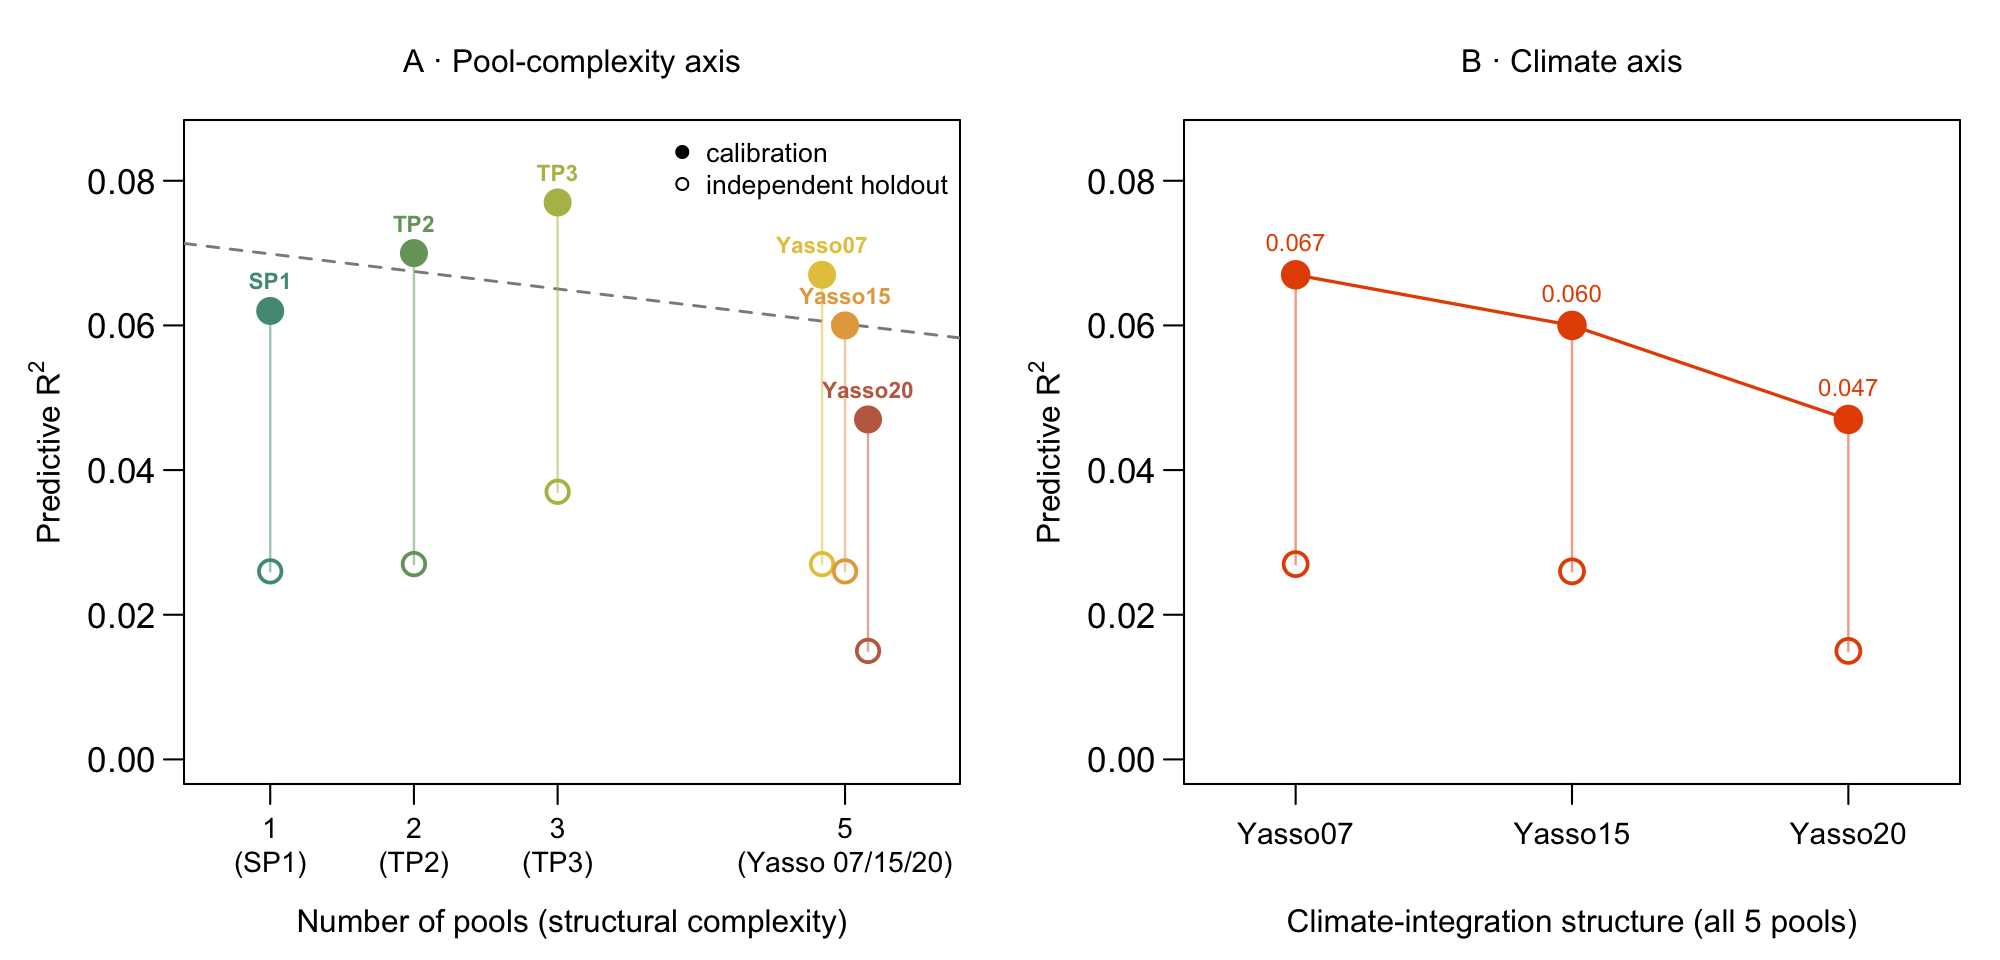
\includegraphics[width=0.98\linewidth]{figures/F6b_skill_vs_complexity.png}\end{center}
\wh{two panels, both $R^2$ (y): \textbf{A} pool count 1$\to$5 (all six), \textbf{B} the climate
sub-axis Yasso07$\to$15$\to$20. Filled = calibration, open = independent holdout.}
\ft{makes ``complexity does not move the answer'' visible in one glance --- the resolution of SIDE ARC~A.
The pool-axis OLS slope is \emph{negative} ($-0.0024\,R^2$/pool); the climate axis falls monotonically
$0.067\!\to\!0.060\!\to\!0.047$; the most complex model (Yasso20) is the worst on both calibration and holdout.}

% =====================================================================
\section*{Action / Results --- what the data can \& cannot constrain (the hinge)}

\paragraph{F7 $\cdot$ KL divergence --- information gain per parameter, the \emph{three Yassos} (merged, rebuilt).}
\begin{center}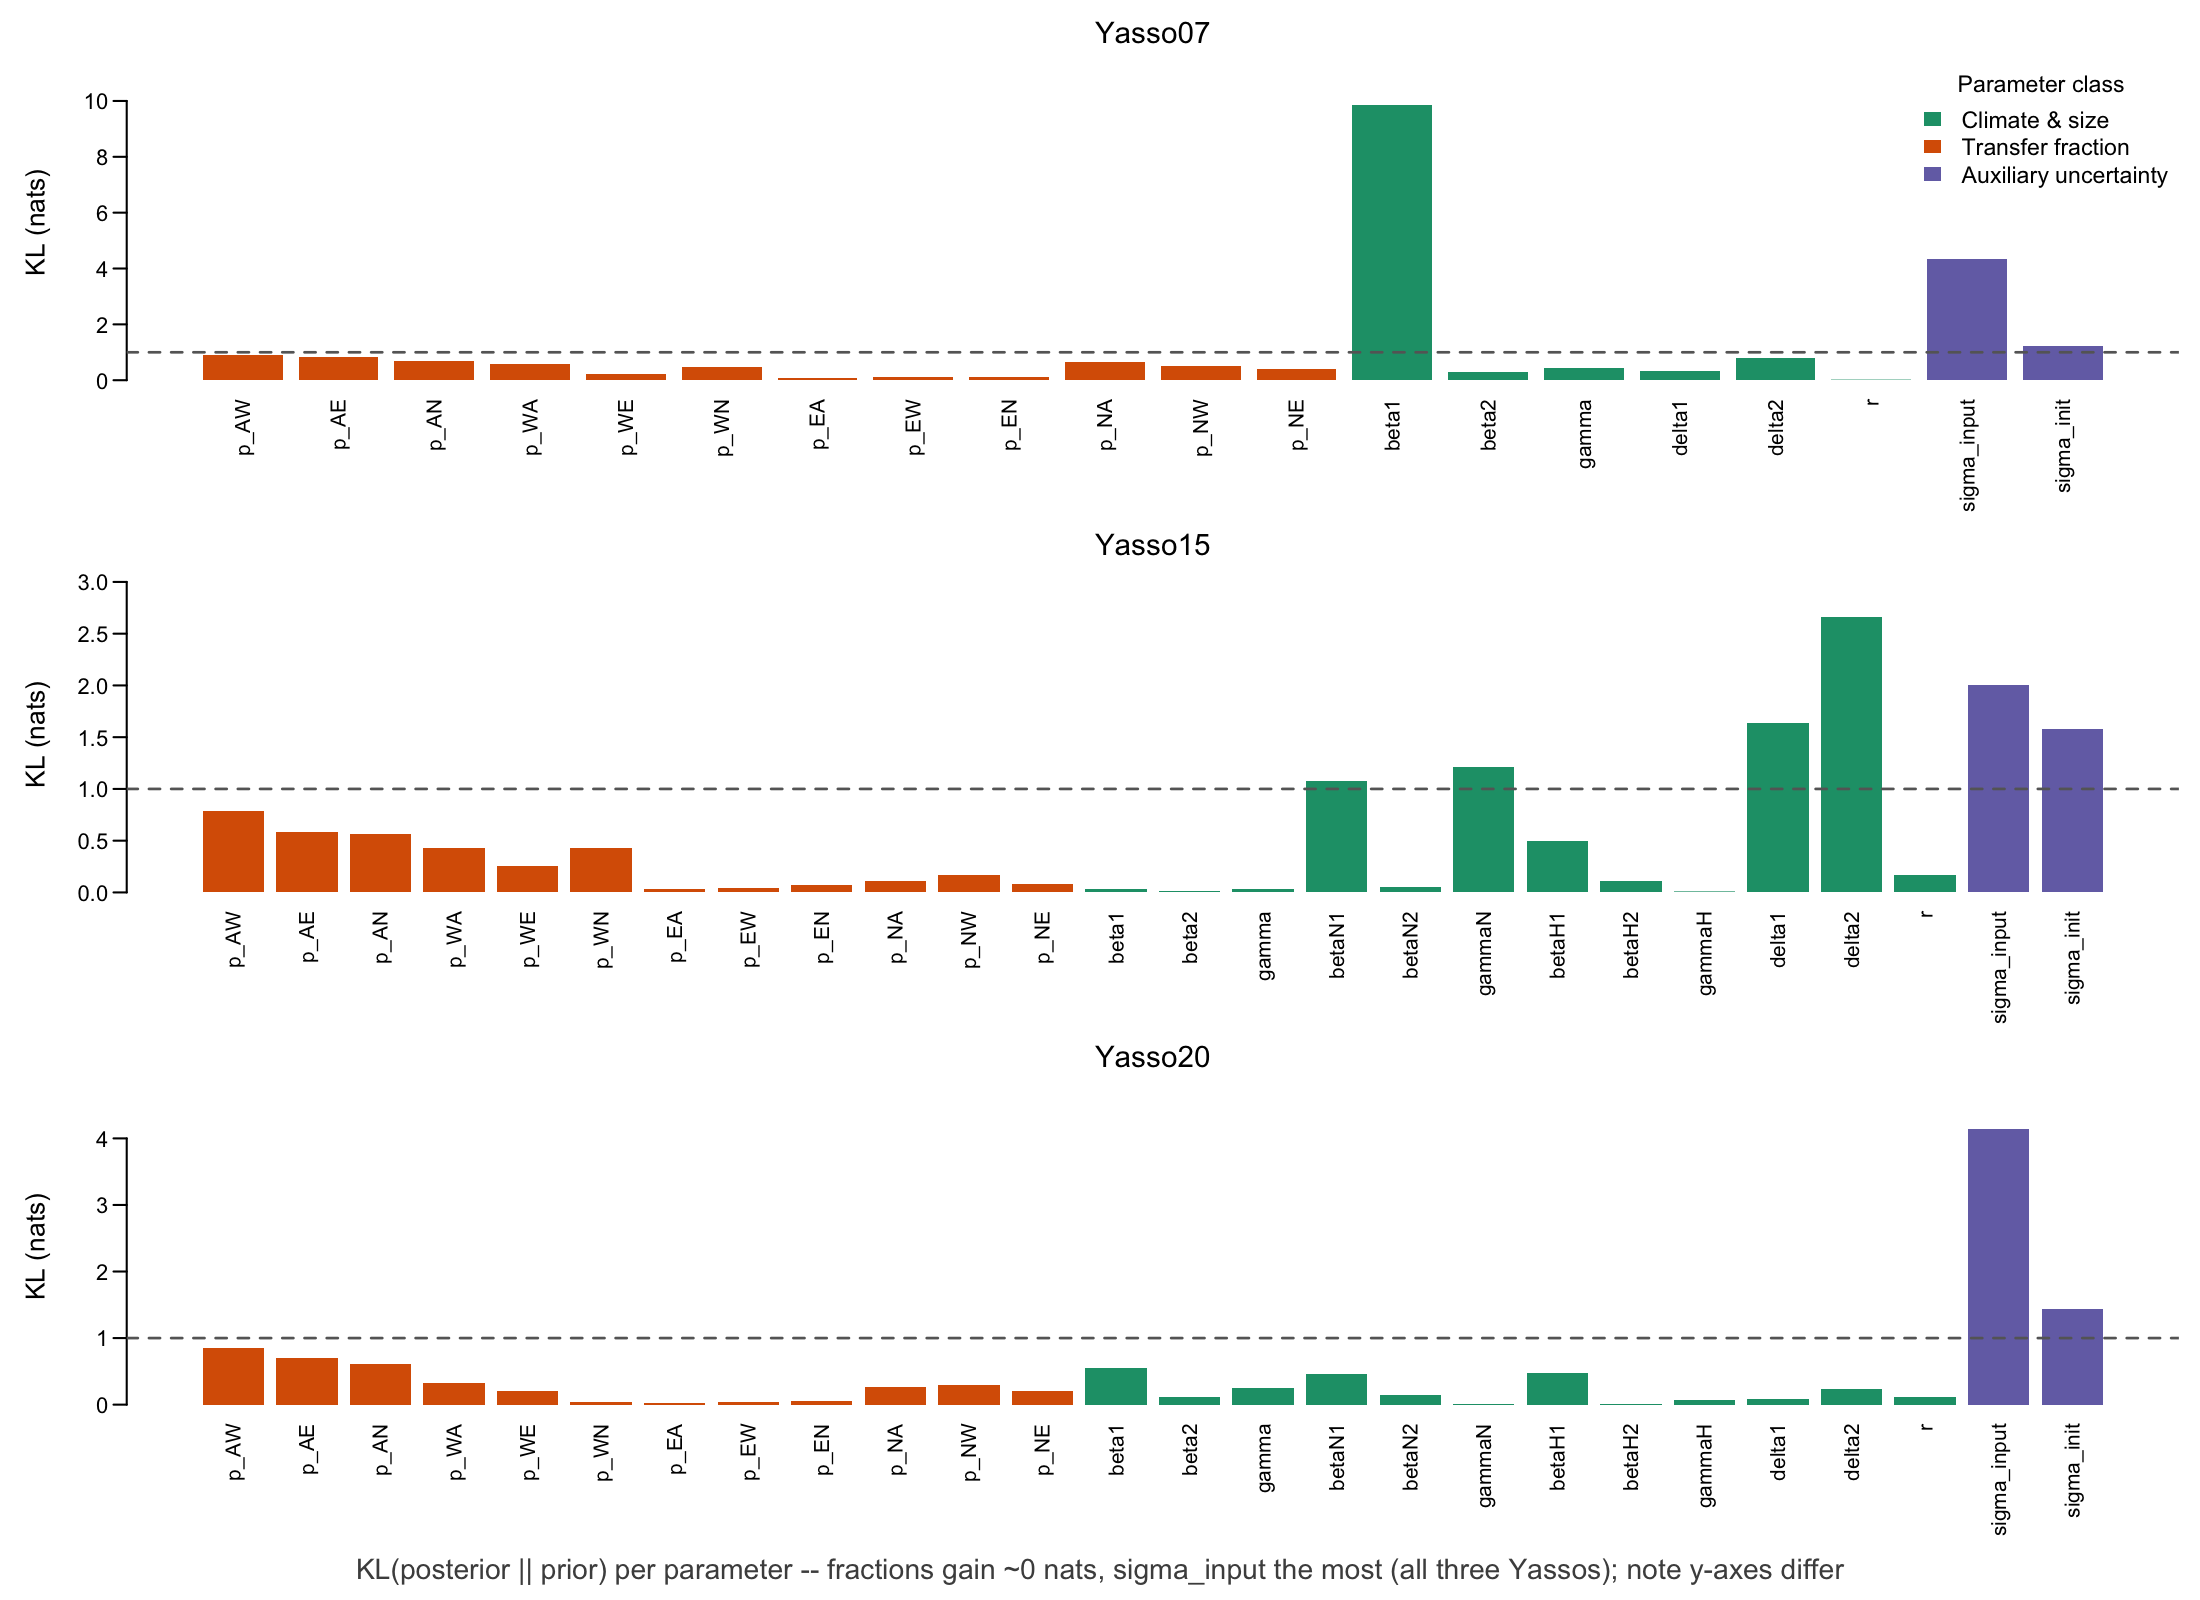
\includegraphics[width=0.86\linewidth]{figures/F7_kl_three_yasso.png}\end{center}
\wh{posterior-vs-prior information gain (nats) per parameter, Yasso07/15/20 as one shared-axis 3-panel plate.
Identical pattern in all three: the 12 transfer \textbf{fractions (orange) gain $\approx$0 nats}, while $\sinput$
(purple) gains the most (up to $\sim$5.5 nats in Yasso20); a few climate/size params (green) gain moderately.
SP1/TP2/TP3 KL $\to$ appendix.}
\ft{data constrains \textbf{inputs, not kinetics}, and it does so \emph{the same way regardless of Yasso variant}
--- the identifiability verdict is structural, not a one-model artefact. The lens that sets up the Trickster
(Side Arc~B) and names the non-identified DoF (F8). \emph{Rebuilt} 2026-07-15 as a faithful KL recompute (posterior
$\times$ engine-reproduced prior) into one clean plate: \texttt{build\_F7F8\_kl\_marginals.R}.}

\paragraph{F8 $\cdot$ Non-identifiability signature --- the fraction trade-off (ridge) structure (Yasso20). (Side Arc~C)}
\begin{center}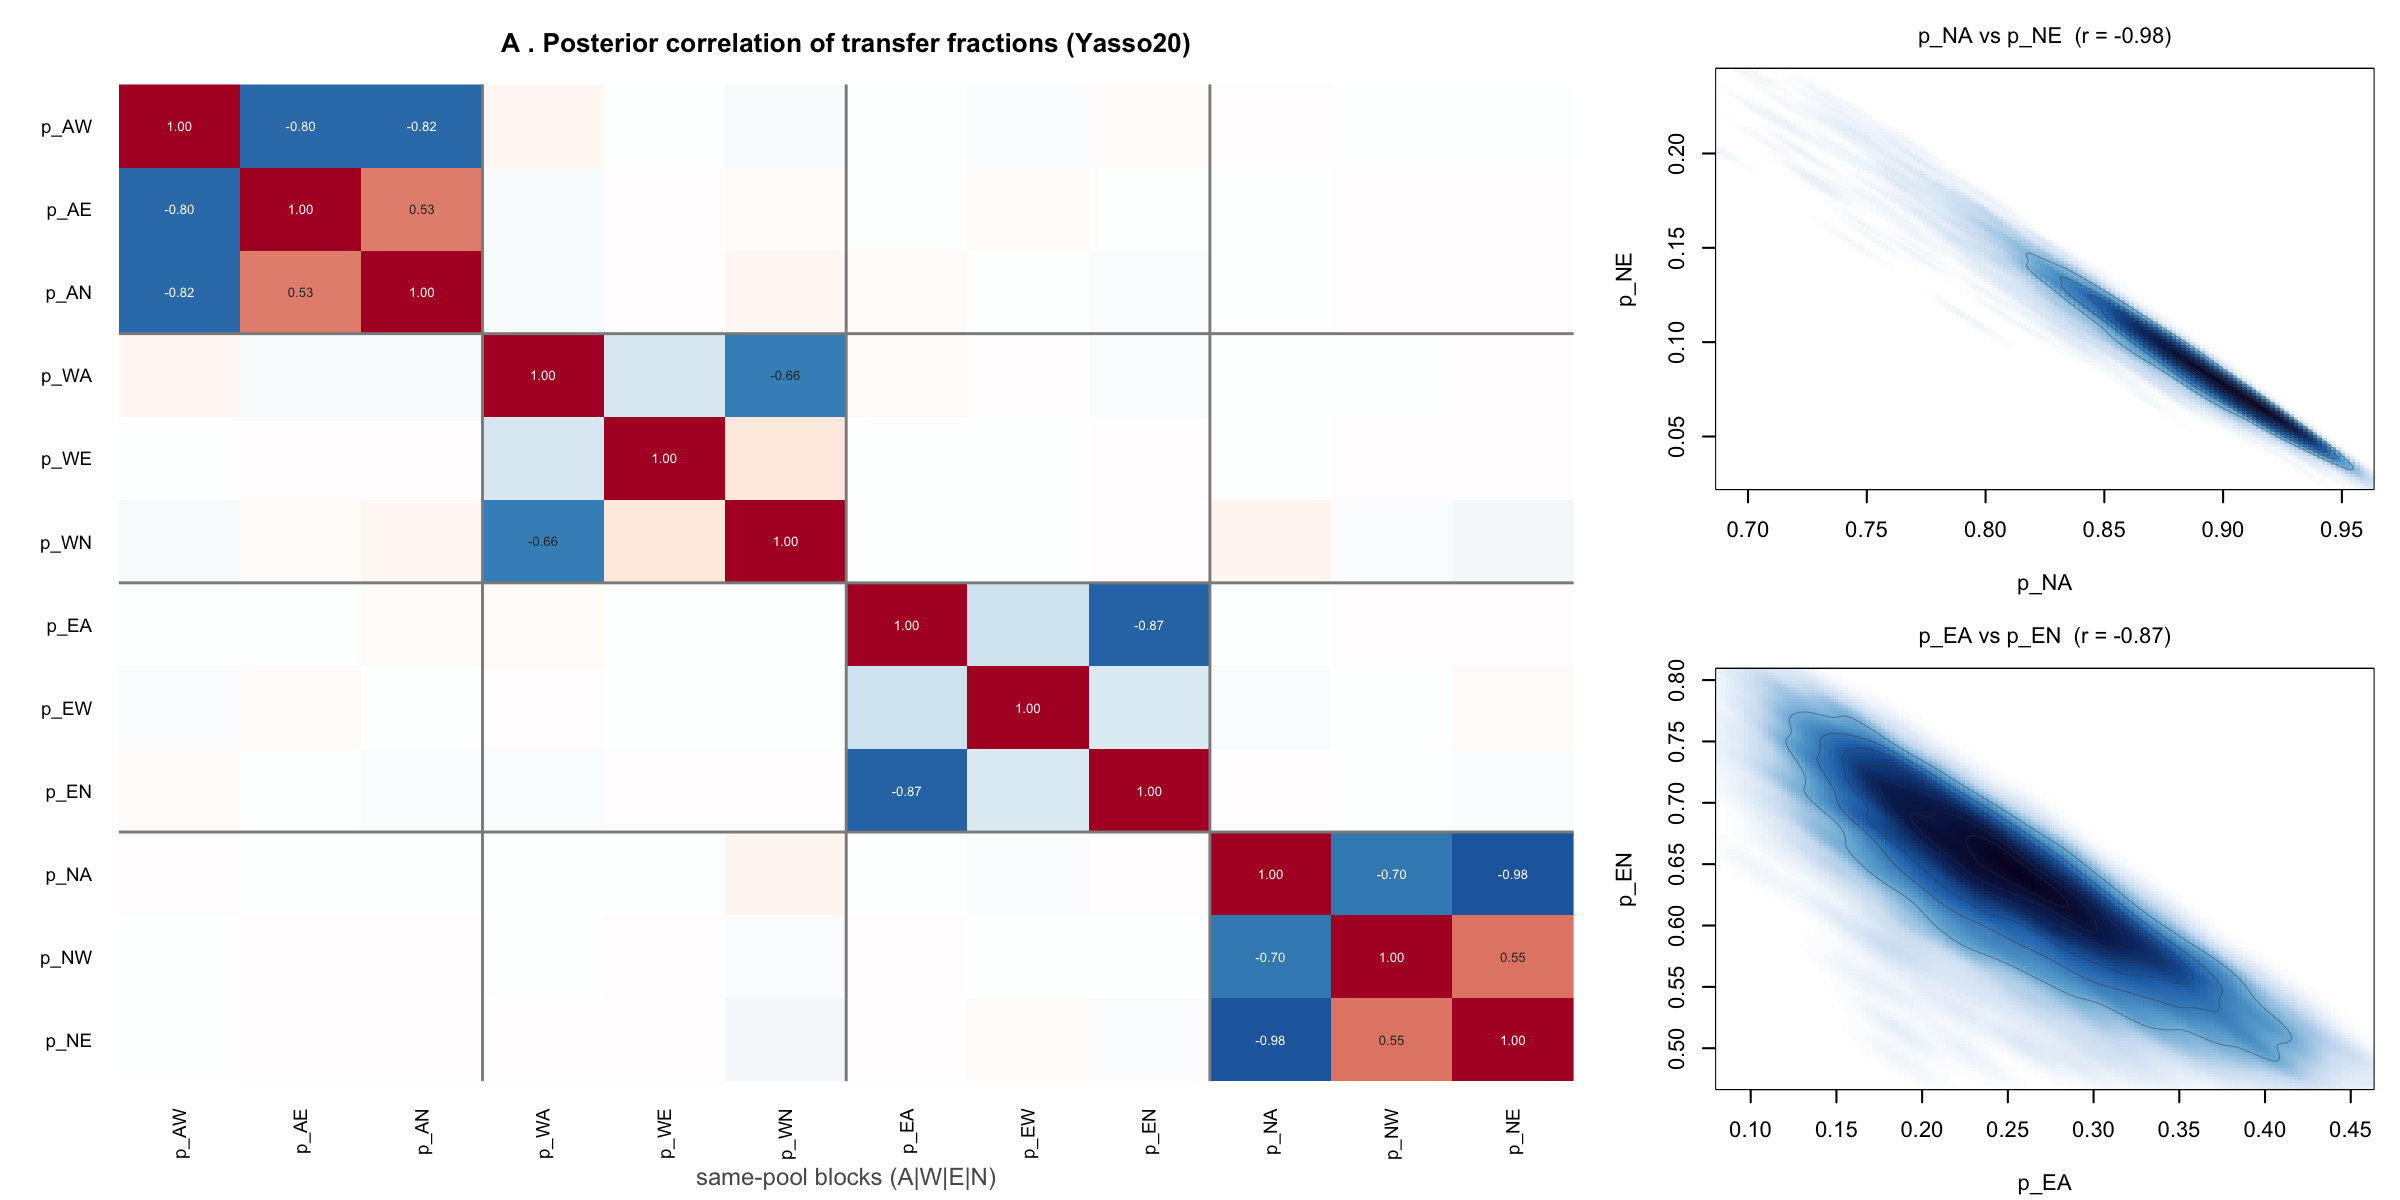
\includegraphics[width=0.98\linewidth]{figures/F8b_fraction_ridges.png}\end{center}
\wh{\textbf{(A)} 12$\times$12 posterior correlation heatmap of the transfer fractions, ordered by source pool. The
block structure is the whole point: fractions leaving the \emph{same} pool anti-correlate near $-1$
(p\_NA$\leftrightarrow$p\_NE $=-0.98$, p\_EA$\leftrightarrow$p\_EN $=-0.86$, p\_AW$\leftrightarrow$p\_AN $=-0.84$),
while \emph{cross}-pool cells are $\approx$0 (white). \textbf{(B)} the two strongest same-pool ridges as continuous
2D density fields (full bandwidth-matrix KDE oriented along the ridge + level curves). Companion table \textbf{T2}
(\texttt{T2\_fraction\_ridges.tex}). \emph{Script:} \texttt{build\_F8b\_fraction\_ridges.R}.}
\ft{``the parameter space is unconstrained'' shown as \emph{geometry}: the data fix only the \textbf{net flux out of
each pool}, not how it splits among destinations --- so each source pool has \emph{one} identified quantity and the
rest is a ridge the posterior slides along. That is the mechanism behind ``complexity buys shape not skill'' (Side
Arc~A) and the KL verdict (F7). \emph{Decision applied 2026-07-15:} this ridge figure is the main Side Arc~C figure;
the old prior-vs-posterior \emph{marginals} are dropped from the main text (Yasso07/15 companions $\to$ appendix
S6). TP3's marginals, where the $\alpha$'s move, belong to the Side Arc~A input-compensation discussion, not here.
\begin{center}\footnotesize% auto-generated by build_F8b_fraction_ridges.R
\begin{tabular}{cccc}
\hline
 Source pool & Fraction pair & Posterior $r$ & Interpretation \\
\hline
N & $p_{NA}\!\leftrightarrow\! p_{NE}$ & -0.98 & net-flux trade-off \\
E & $p_{EA}\!\leftrightarrow\! p_{EN}$ & -0.88 & net-flux trade-off \\
A & $p_{AW}\!\leftrightarrow\! p_{AN}$ & -0.83 & net-flux trade-off \\
A & $p_{AW}\!\leftrightarrow\! p_{AE}$ & -0.79 & net-flux trade-off \\
N & $p_{NA}\!\leftrightarrow\! p_{NW}$ & -0.69 & net-flux trade-off \\
E & $p_{EA}\!\leftrightarrow\! p_{EW}$ & -0.31 & net-flux trade-off \\
\hline
\end{tabular}
\normalsize\end{center}}

% =====================================================================
\section*{Resolution / Discussion --- the auxiliary-$\sigma$ reveal ($\sinput$ \& $\sinit$; Trickster payoff)}

\paragraph{F9 $\cdot$ The two auxiliary uncertainty parameters, one plate ($\sinput$ $|$ $\sinit$). (MERGED F9+F10, bounded-only)}
\begin{center}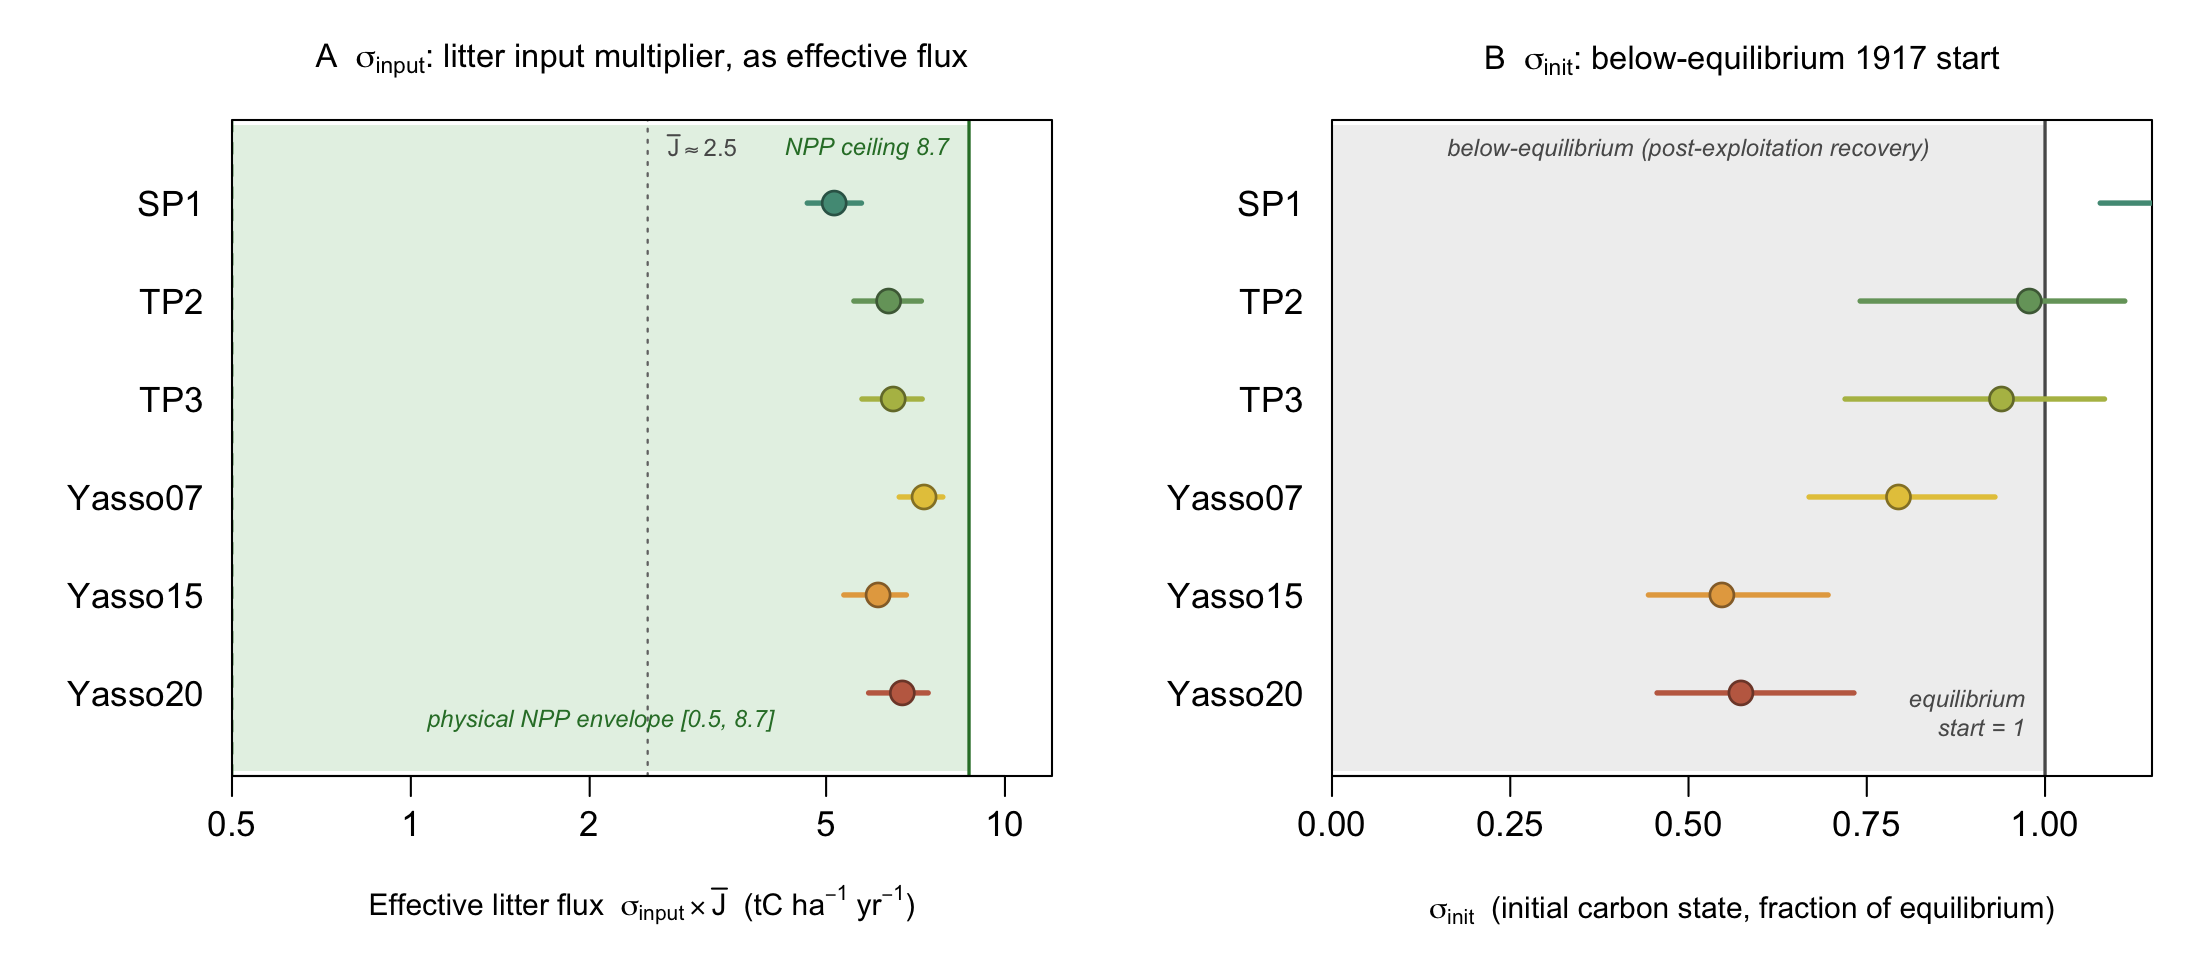
\includegraphics[width=0.98\linewidth]{figures/F9_auxiliary_sigmas.png}\end{center}
\wh{two matched per-model forest plots. \textbf{(a)} $\sinput$ as effective litter flux $\sinput\times\bar{J}$
against the green \emph{physical NPP envelope} [0.5, 8.7]\,tC\,ha$^{-1}$\,yr$^{-1}$ --- under the flux bound all
six sit inside it (0.9--6.3). \textbf{(b)} $\sinit$ as the initial carbon state (fraction of equilibrium);
every 95\% interval lies below the reference line at 1. Points/whiskers use the per-model palette
(consistent with F4).}
\ft{the two auxiliary parameters are \emph{both physically interpretable} once bounded: $\sinput$ within the
NPP envelope (no manufactured carbon), $\sinit<1$ = a below-equilibrium 1917 start (post-exploitation recovery,
the [History] thread). Two-pool models lean hardest ($\sinit$ 0.15--0.24) vs Yasso (0.5--0.7). \emph{Only the
flux-bounded run appears in the main story} (decision 2026-07-14, option~B); the unbounded ``before'' run ---
where TP2/TP3 blow through to 34/50 --- is a diagnostic in the \emph{physically-bounded input priors} appendix
(\texttt{appendix\_sigma\_input.tex}, keeps \texttt{build\_F9\_effective\_flux.R} + its before/after figure), NOT
a second reported pipeline. Merged fig script: \texttt{build\_F9\_auxiliary\_sigmas.R}.}

\paragraph{F10b $\cdot$ Finnish forest history --- post-war exploitation $\to$ managed growth ([History] thread).}
\begin{center}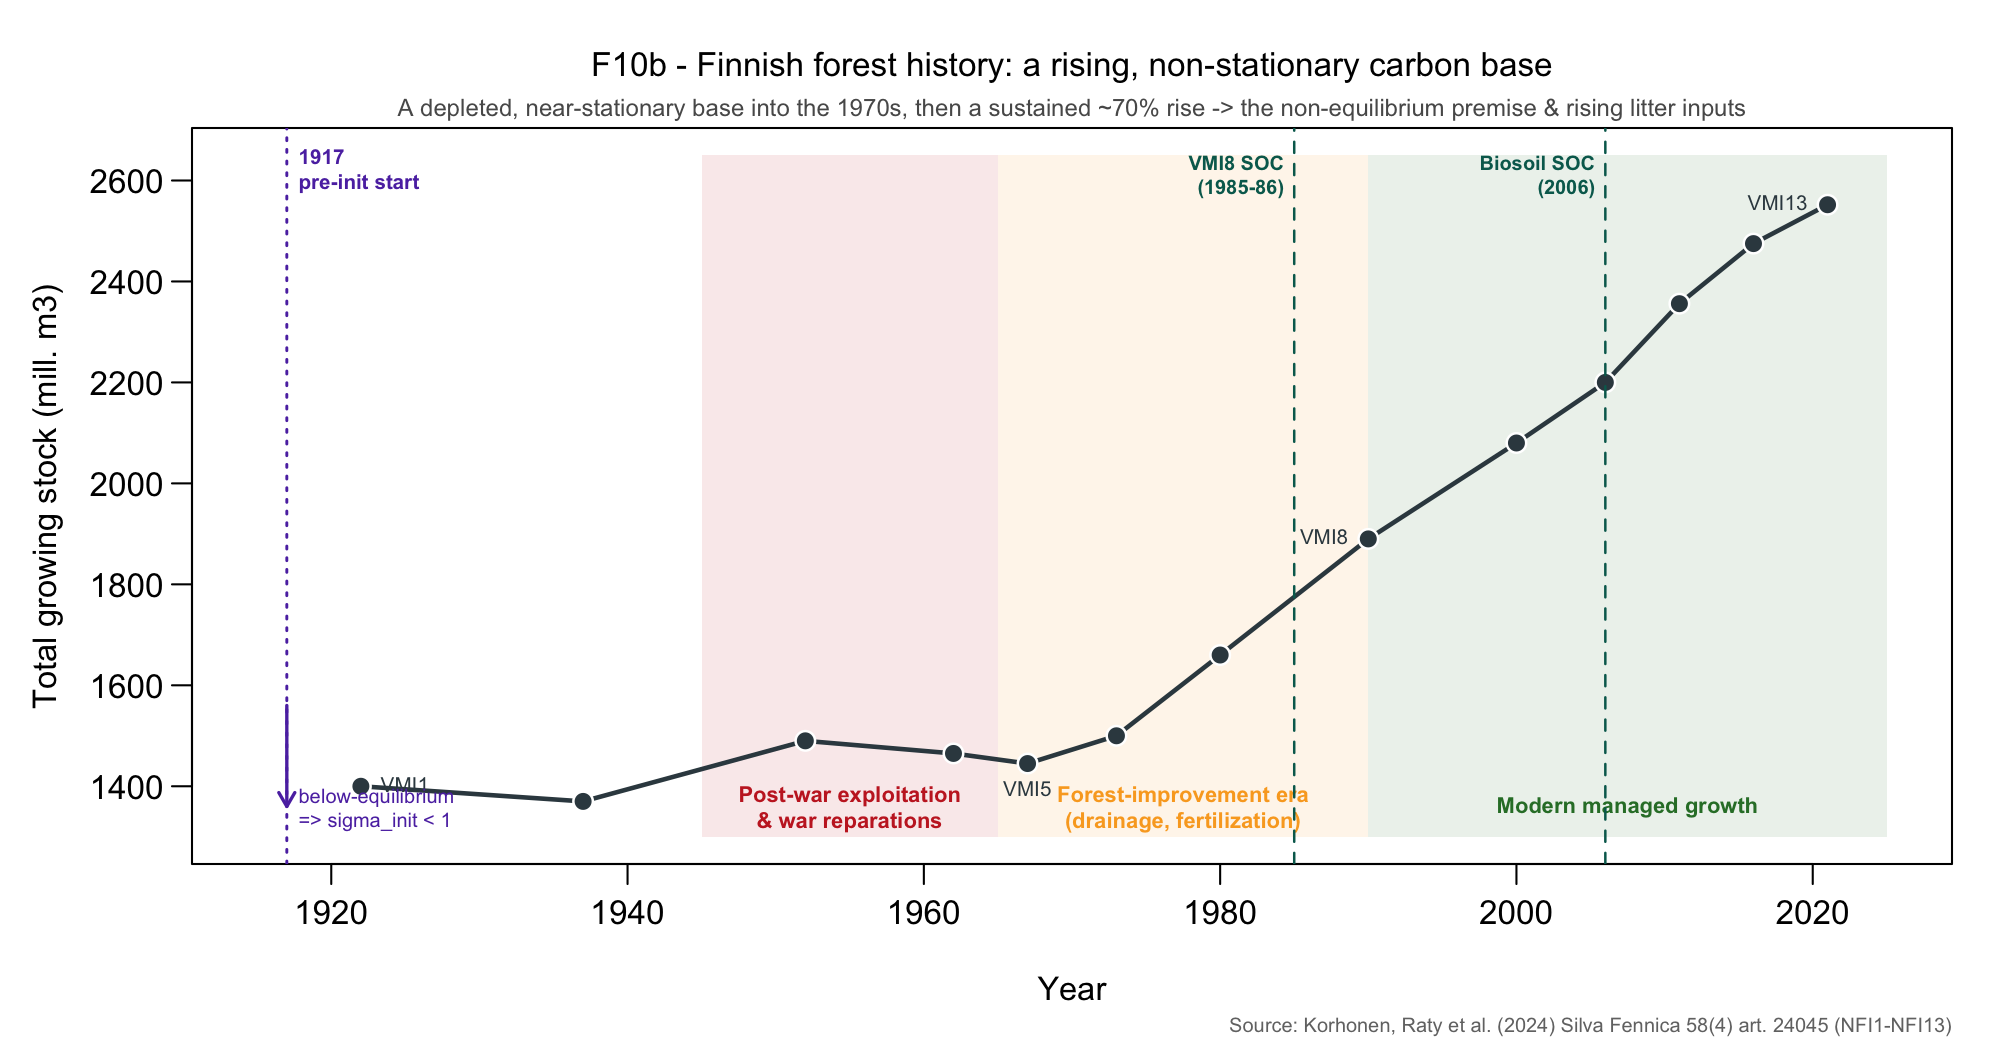
\includegraphics[width=0.95\linewidth]{figures/F10b_forest_history.png}\end{center}
\wh{NFI total growing stock (VMI1--VMI13): a depleted, near-stationary base into the 1970s, then a sustained
$\sim$70\% rise, across three management eras; the 1917 pre-init anchor and the VMI8/Biosoil SOC campaigns marked.
\emph{Source: Korhonen, R\"aty et al. (2024) Silva Fennica 58(4) art.~24045 (anchors NFI1/11/12/13 quoted; NFI2--NFI10
from the paper's Fig.~10 development curve).}}
\ft{the \emph{physical justification} for the non-equilibrium premise and the rising, non-stationary input history --- why $\sinit<1$ and why contemporary litter rises (F1). The [History] thread made concrete exactly where we discuss inputs.}

% =====================================================================
\section*{Resolution --- residual structure \& where to go next (the frontier)}
\textit{Not a loose end but the \textbf{frontier arc}: the residual structure names \emph{where} the recoverable
signal still hides, and it points in the same direction as the whole paper --- the forcing, not the kinetics.}

\paragraph{F11 $\cdot$ RF importance heatmap (residual drivers) --- the ``where to go next'' figure (rebuilt, formatted labels).}
\begin{center}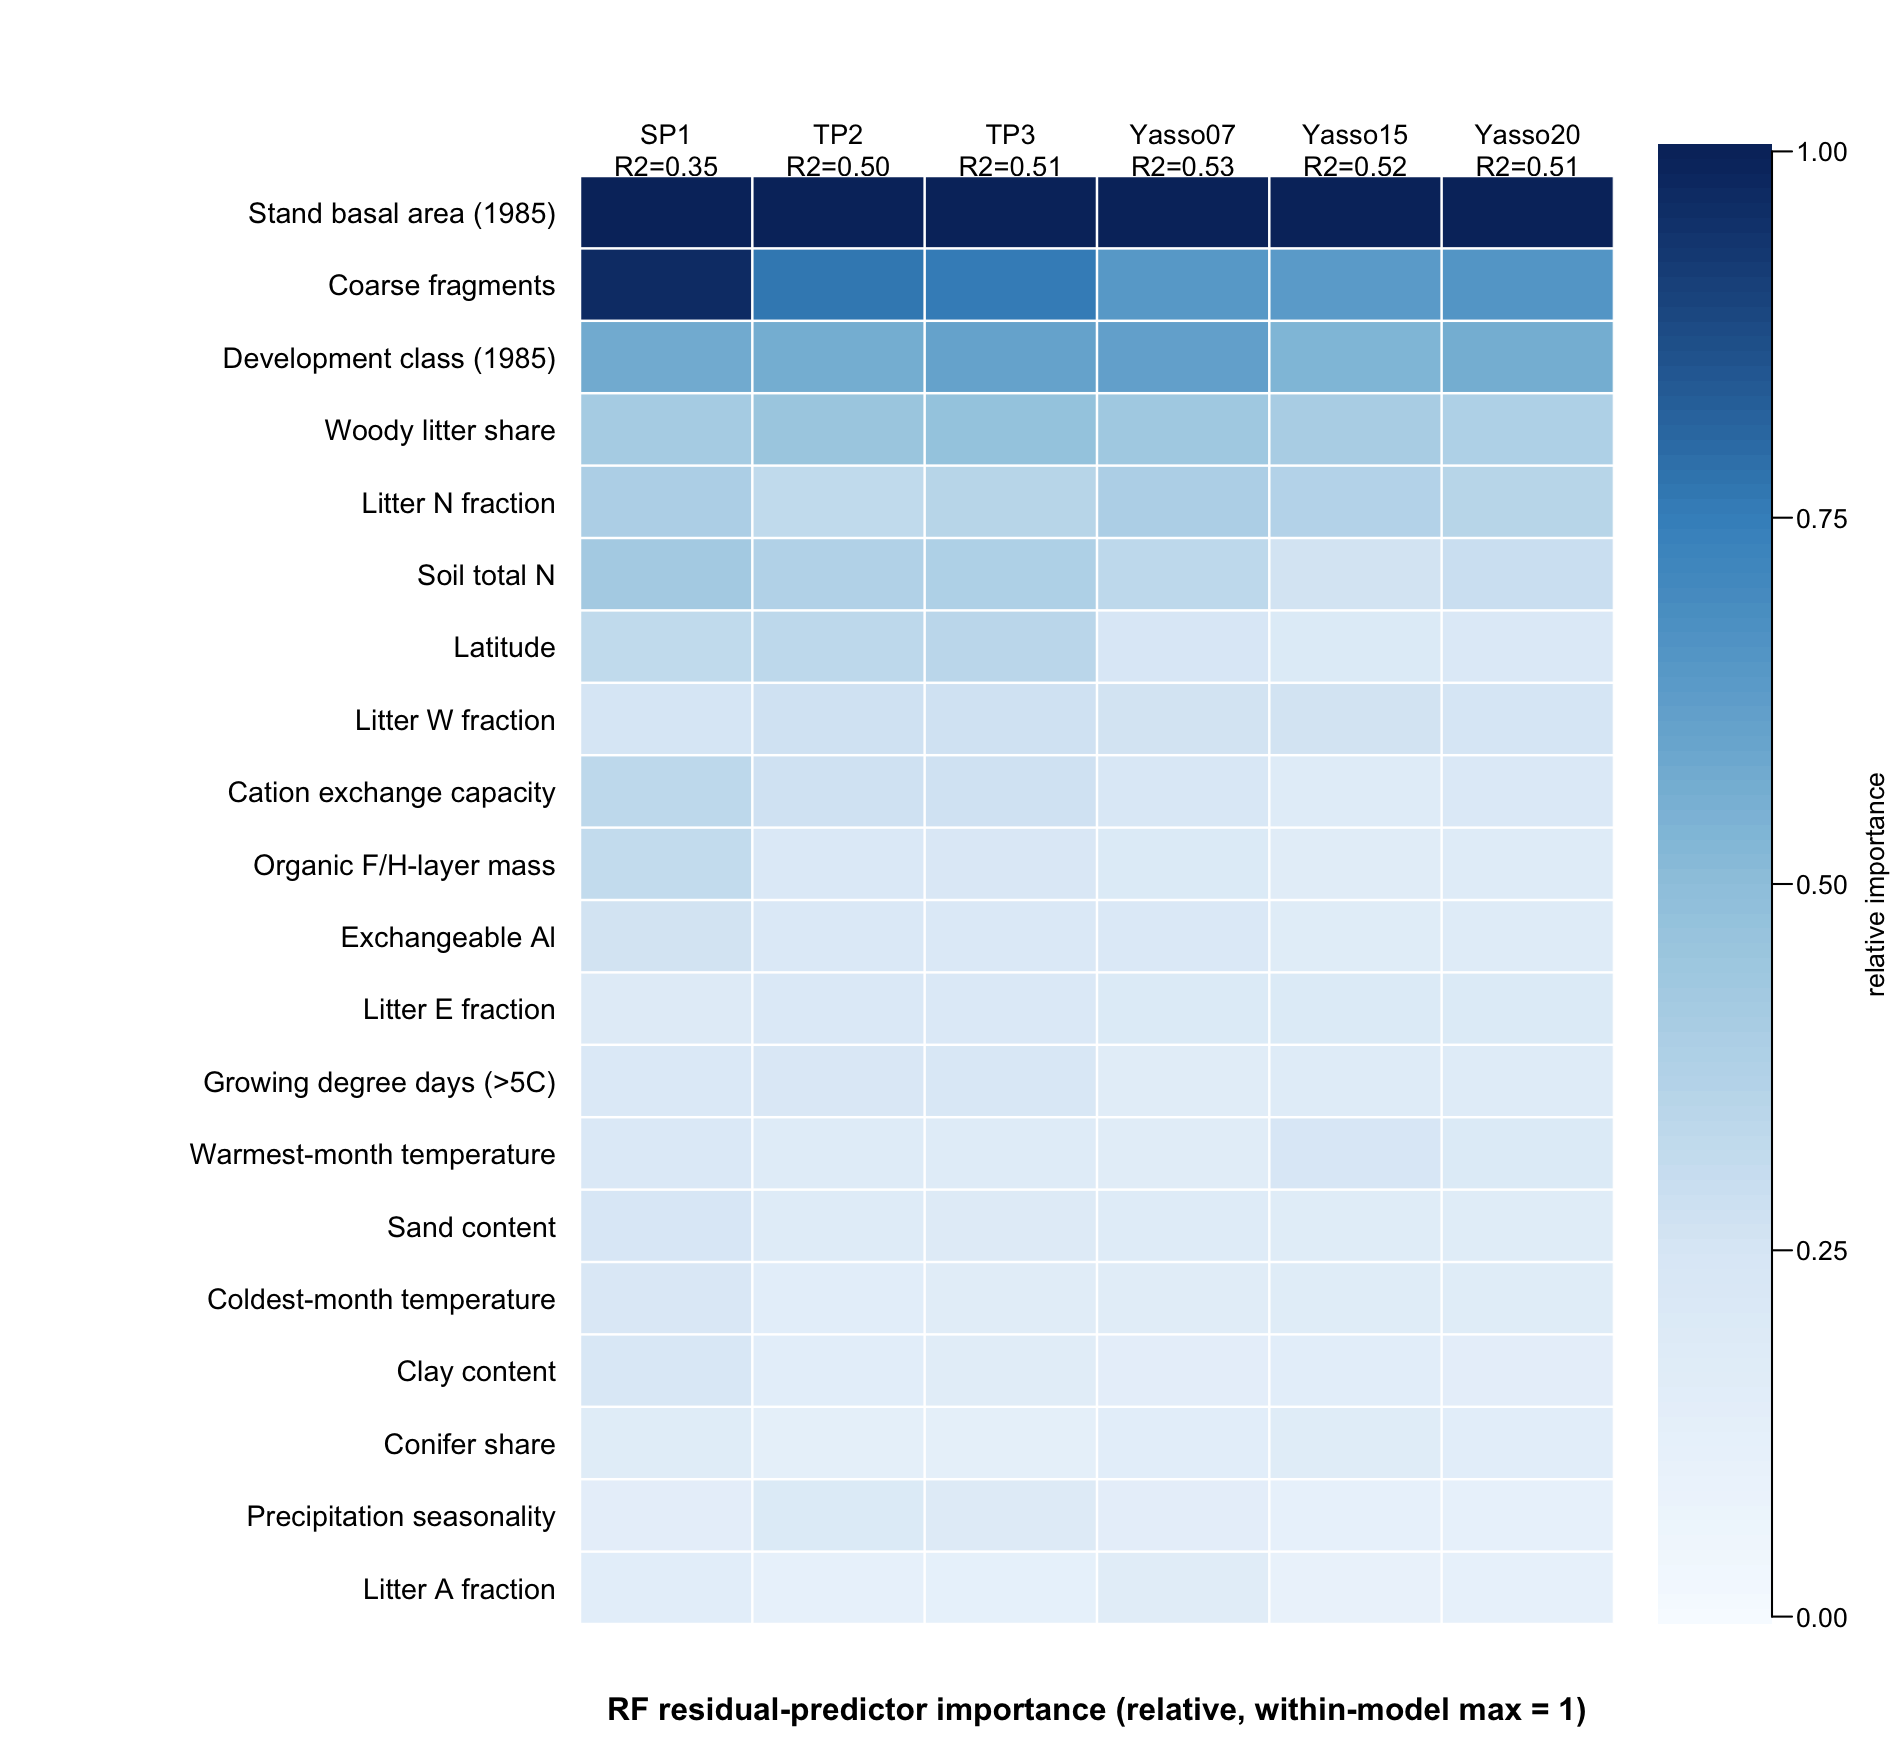
\includegraphics[width=0.8\linewidth]{figures/F11_rf_heatmap.png}\end{center}
\wh{random-forest importances for the plot-level residuals (relative, within-model max = 1; rows = union of each
model's top-15, readable predictor names). \textbf{Stand basal area is the leading, diffuse, shared driver}
(top in \emph{all six} models), soil total N + cation exchange + climate next, each individually smaller.
The ordering is \emph{consistent across all six structures}; per-model OOB $R^2$ 0.34--0.43 in the column headers.
\emph{Script:} \texttt{build\_F11\_rf\_heatmap.R}.}
\ft{the frontier beat, and it closes the loop. That basal area --- a \textbf{productivity/input} proxy --- leads
the residual in \emph{every} model (not a kinetic or pool variable) says the recoverable signal that remains lives
in the \textbf{forcing}, exactly where Side Arc~B put the binding uncertainty and where F6's basal-area classing
already hinted. So the two-pronged frontier follows directly: (i) reconstruct the input \emph{history} (temporal),
(ii) stratify the input \emph{level} by site class (spatial --- the optional red strand), both bounded by the same
physical envelope. The one thing it does \emph{not} motivate is adding kinetic complexity --- the surplus DoF there
are already non-identified (F7/F8). ``Where to go next'' = better forcing, not a bigger model.}

% =====================================================================
\section*{Application / Policy --- wall-to-wall SOC (NextGenC)}
\textit{The policy-relevant deliverable: the operational product feeding the Finnish GHG inventory.}

\paragraph{F12 $\cdot$ National wall-to-wall SOC --- ensemble mean stock \emph{and} cross-model uncertainty (one plate, 2 panels).}
\begin{center}

\includegraphics[width=0.49\linewidth]{\rep/SOC_maps/thumbnails/ENSEMBLE_SOC_mean.png}\hfill

\includegraphics[width=0.49\linewidth]{\rep/SOC_maps/thumbnails/ENSEMBLE_SOC_sd.png}
\end{center}
\wh{\textbf{(a)} kriged 2 km ensemble-mean SOC over Finland --- south-high/north-low gradient (black = peat/water
masked); \textbf{(b)} the between-model spread per cell --- where the six structures agree and where they don't.
Merged from the former F12 (mean) + F13 (SD).}
\ft{the headline policy output (a wall-to-wall SOC stock estimate) paired with its honest, spatial uncertainty ---
panel (b) is the spatial face of ``structure is a weak lever'' (modest, structured spread), read against the stock in (a).}

\paragraph{F13 $\cdot$ SOC dynamics --- current change \emph{and} stabilization state (one plate, 2 panels).}
\begin{center}

\includegraphics[width=0.49\linewidth]{\rep/SOC_maps/thumbnails/ENSEMBLE_SOC_delta10yr.png}\hfill

\includegraphics[width=0.49\linewidth]{\rep/SOC_maps/thumbnails/ENSEMBLE_vulnerability.png}
\end{center}
\wh{\textbf{(a)} wall-to-wall 10-yr SOC change (ensemble OLS slope 2015--2024) --- gaining (blue) vs losing (red);
\textbf{(b)} the \emph{stabilization state} of the carbon $=$ Yasso-ensemble \textbf{labile (less-stabilized) SOC
fraction} $(A{+}W{+}E)/$total, 2015--2024 mean (\emph{Yasso subset only} --- the simple models have no pool
partition). Both kriged at 2 km, peat black.}
\ft{two \emph{different} axes of soil-carbon dynamics. (a) is the current trajectory; (b) is \emph{how} the carbon
is held --- fast-cycling, less-processed material (high, north) vs.\ humified legacy carbon (low, south). \textbf{We
deliberately do NOT label (b) a ``vulnerability'' or ``warming-sensitivity'' map:} the carbon-quality--temperature
relationship (recalcitrant SOC has the higher Q$_{10}$) makes the sign of any such reading contested, and Yasso
scales $\xi$ uniformly across pools. The defensible, sign-neutral reading is descriptive --- \emph{stabilization/
turnover state} --- and its storyline hook is \textbf{inputs, not climate}: the labile pool tracks recent litter,
so high-labile soils are those whose stock is set by \emph{contemporary inputs} (on-spine with the init/inputs
thesis; humus-rich soils are legacy/history-dominated). \emph{Prototype 2026-07-15:} only partly correlated with
$\Delta$SOC ($r{=}0.48$, $\rho{=}0.64$, $R^2{=}0.23$) $\Rightarrow$ a distinct signal (dynamic soils change more).
The pool partition is itself model-structural (where structure differs, non-identified) --- on-thesis, and a
manuscript version should show the between-Yasso spread. \emph{Script:} \texttt{build\_vulnerability\_map.R}
(kriged, EPSG:3035, NextGenC pipeline).}

% =====================================================================
\section*{Supplementary figures (sanity / robustness --- out of the main flow)}
\textit{Support the main claims but not part of the narrative spine; collected here for the supplement.}

\paragraph{S1 (was F5) $\cdot$ Per-plot SOC trajectories (physical-sanity).}
\begin{center}
\includegraphics[width=0.9\linewidth]{\rep/NextGenC_SOC_trajectories.png}\end{center}
\wh{every plot's mean SOC; all models now peak at a physical $\sim$100 tC/ha; TP2/TP3 jagged, SP1 smooth.}
\ft{shows the flux bound worked (no inflated stocks) and that the TP3 oscillation is a real fast-pool signal, not
the old Euler artefact. Moved out of the main results (2026-07-15): it is a robustness check, not a spine beat.
The rest of the robustness triage is now built as S3--S6 (convergence, residuals, non-Yasso KL, ridge companions);
the TP3 exact-vs-Euler integrator check was dropped.}

\paragraph{S2 (was F6 calibration half) $\cdot$ Observed vs predicted --- CALIBRATION plots (recoloured).}
\begin{center}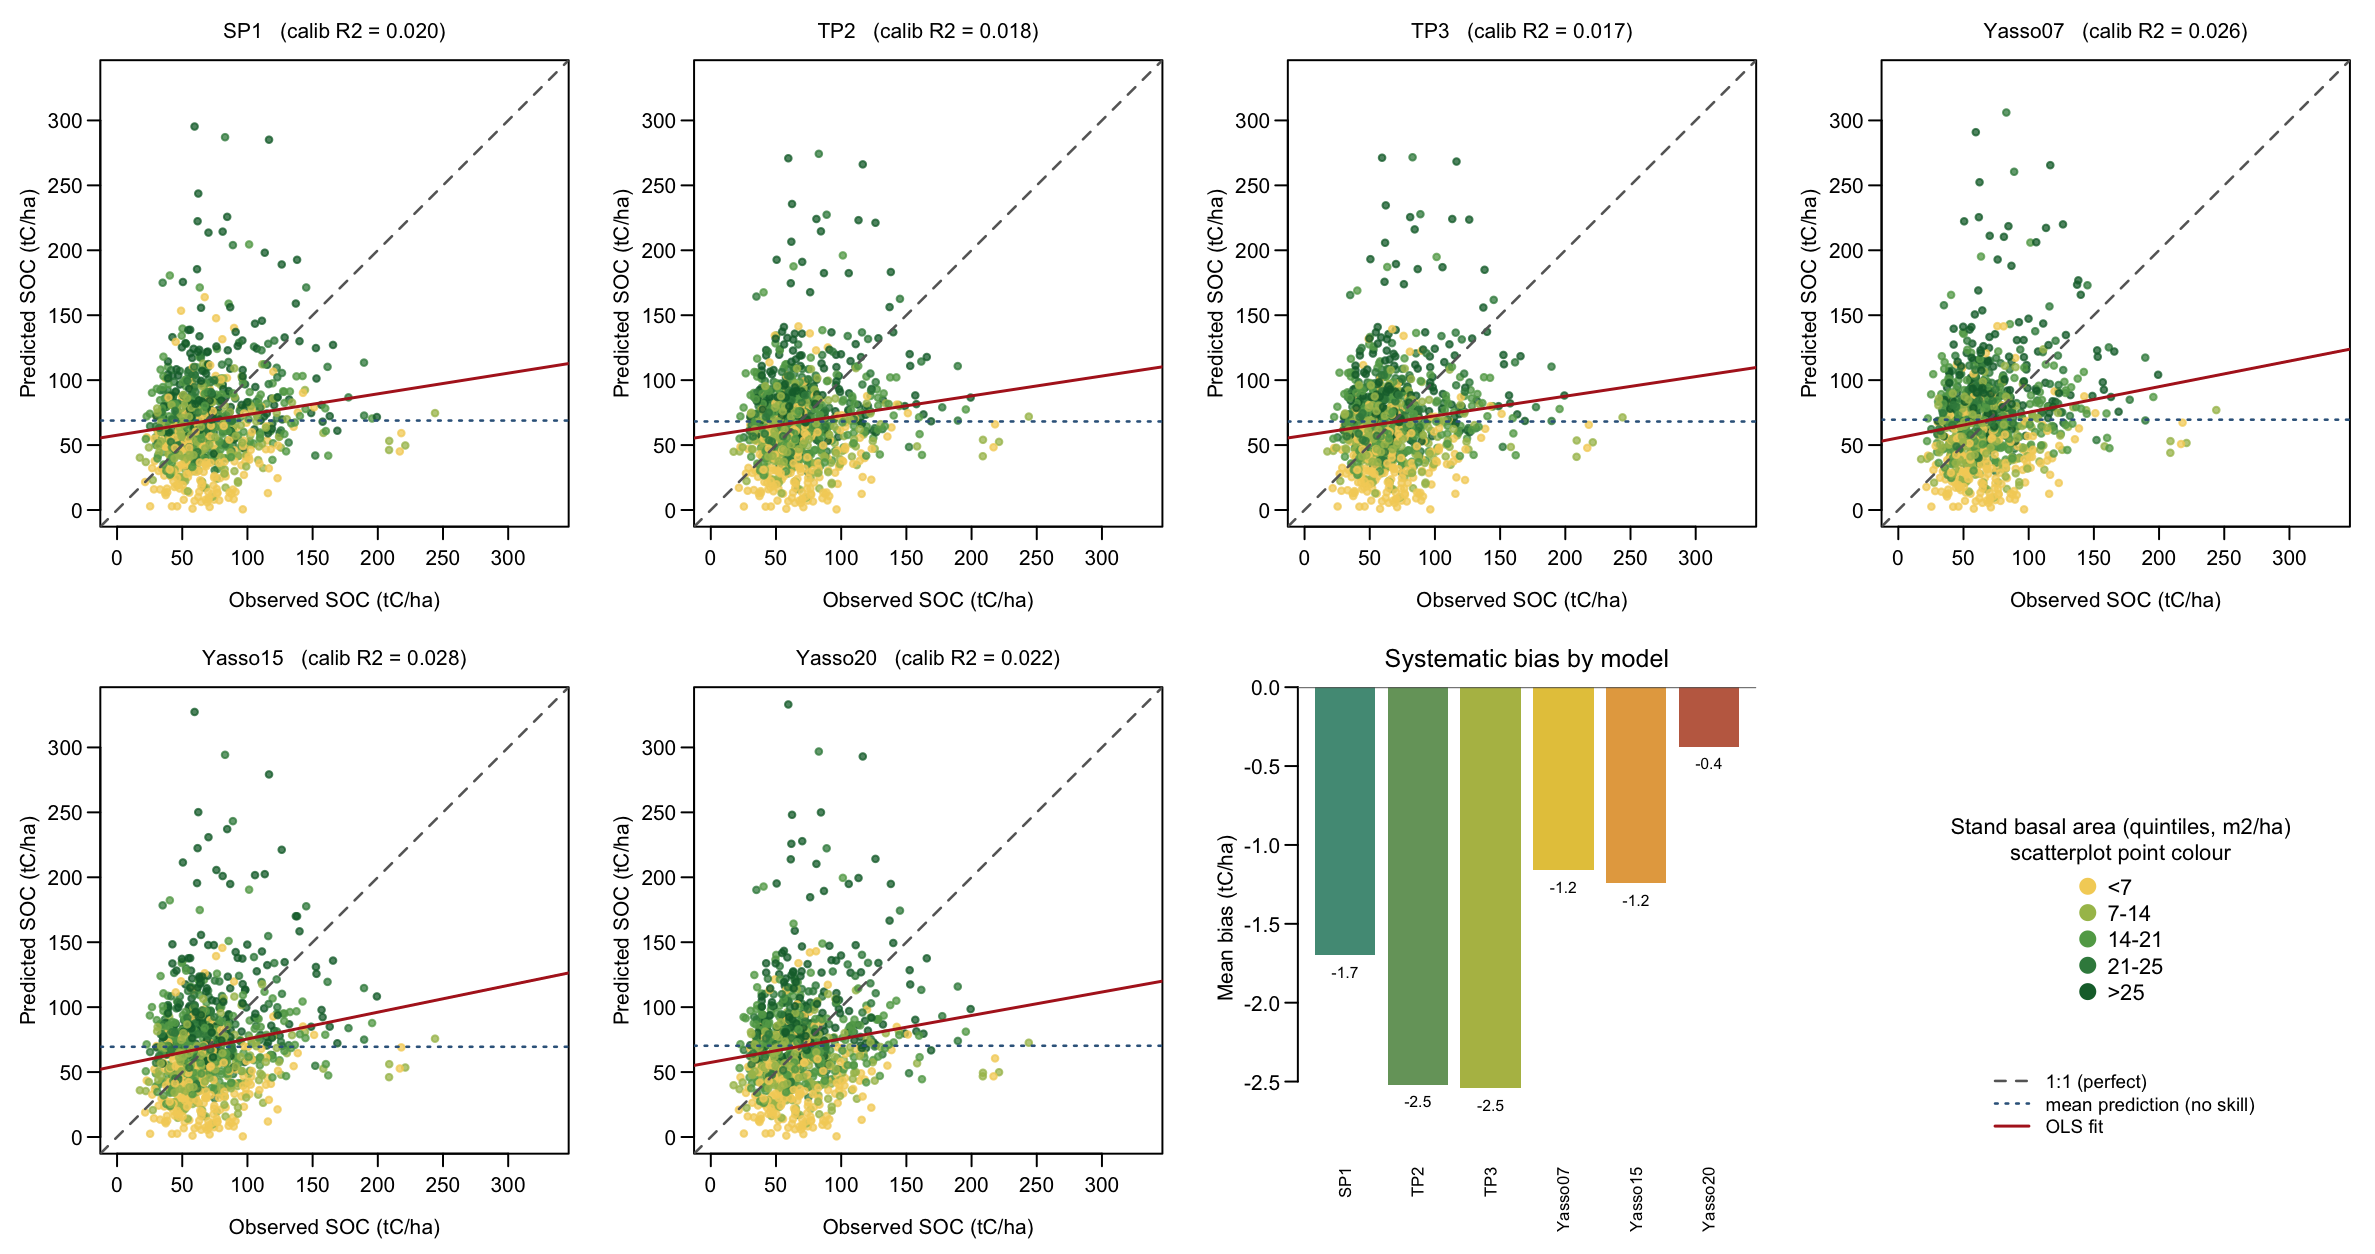
\includegraphics[width=0.98\linewidth]{figures/S2_obs_vs_pred_calib.png}\end{center}
\wh{the in-sample companion to the main-text holdout F6: six calibration obs-vs-pred scatterplots + a
systematic-bias barplot. \textbf{Colour coding (2026-07-15):} the scatterplots use the \emph{same basal-area
quintile palette as F6} (Green-Gold); the bias barplot uses the \emph{shared per-model palette} (Temperature
Diverging), matching every other by-model figure. Calib $R^2$ 0.062--0.077. \emph{Script:} \texttt{build\_S2\_obs\_vs\_pred\_calib.R}.}
\ft{kept in the supplement so the main figure (F6) carries only the honest out-of-sample panel. Same small
between-model spread, one notch higher than holdout; bias climbs mildly with over-prediction (Yasso20 highest).}

\textit{--- Robustness set (built 2026-07-15; the ``robustness triage'' appendix) ---}

\paragraph{S3 $\cdot$ MCMC convergence.}
\begin{center}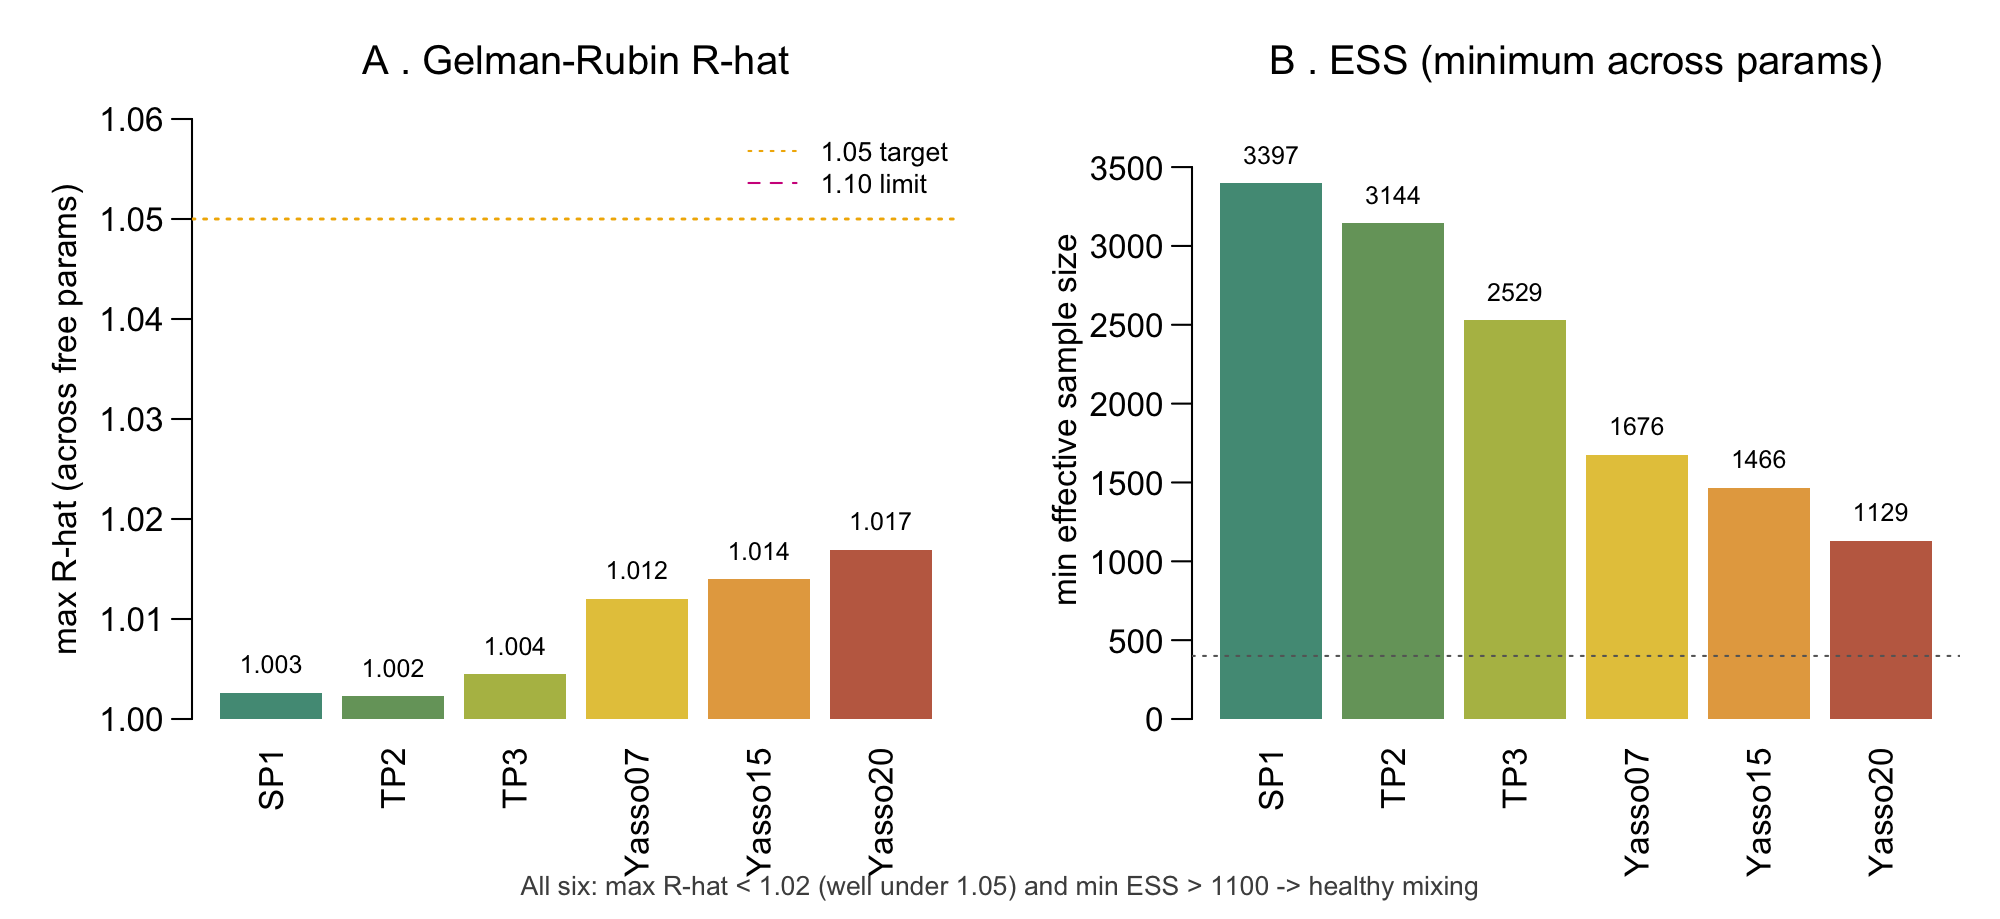
\includegraphics[width=0.85\linewidth]{figures/R1_convergence.png}\end{center}
\wh{per-model \textbf{(A)} max R-hat and \textbf{(B)} min ESS across all free parameters. All six: max R-hat
$<$1.02 (well under the 1.05 target) and min ESS $>$1100. \emph{Script:} \texttt{build\_robustness\_conv\_resid.R}.}
\ft{the sampler converged everywhere --- so good fraction R-hat reflects healthy \emph{mixing}, not identifiability
(the non-identifiability shows up in KL / prior-pinning, F7/F8, not in R-hat).}

\paragraph{S4 $\cdot$ Residual diagnostics (pooled).}
\begin{center}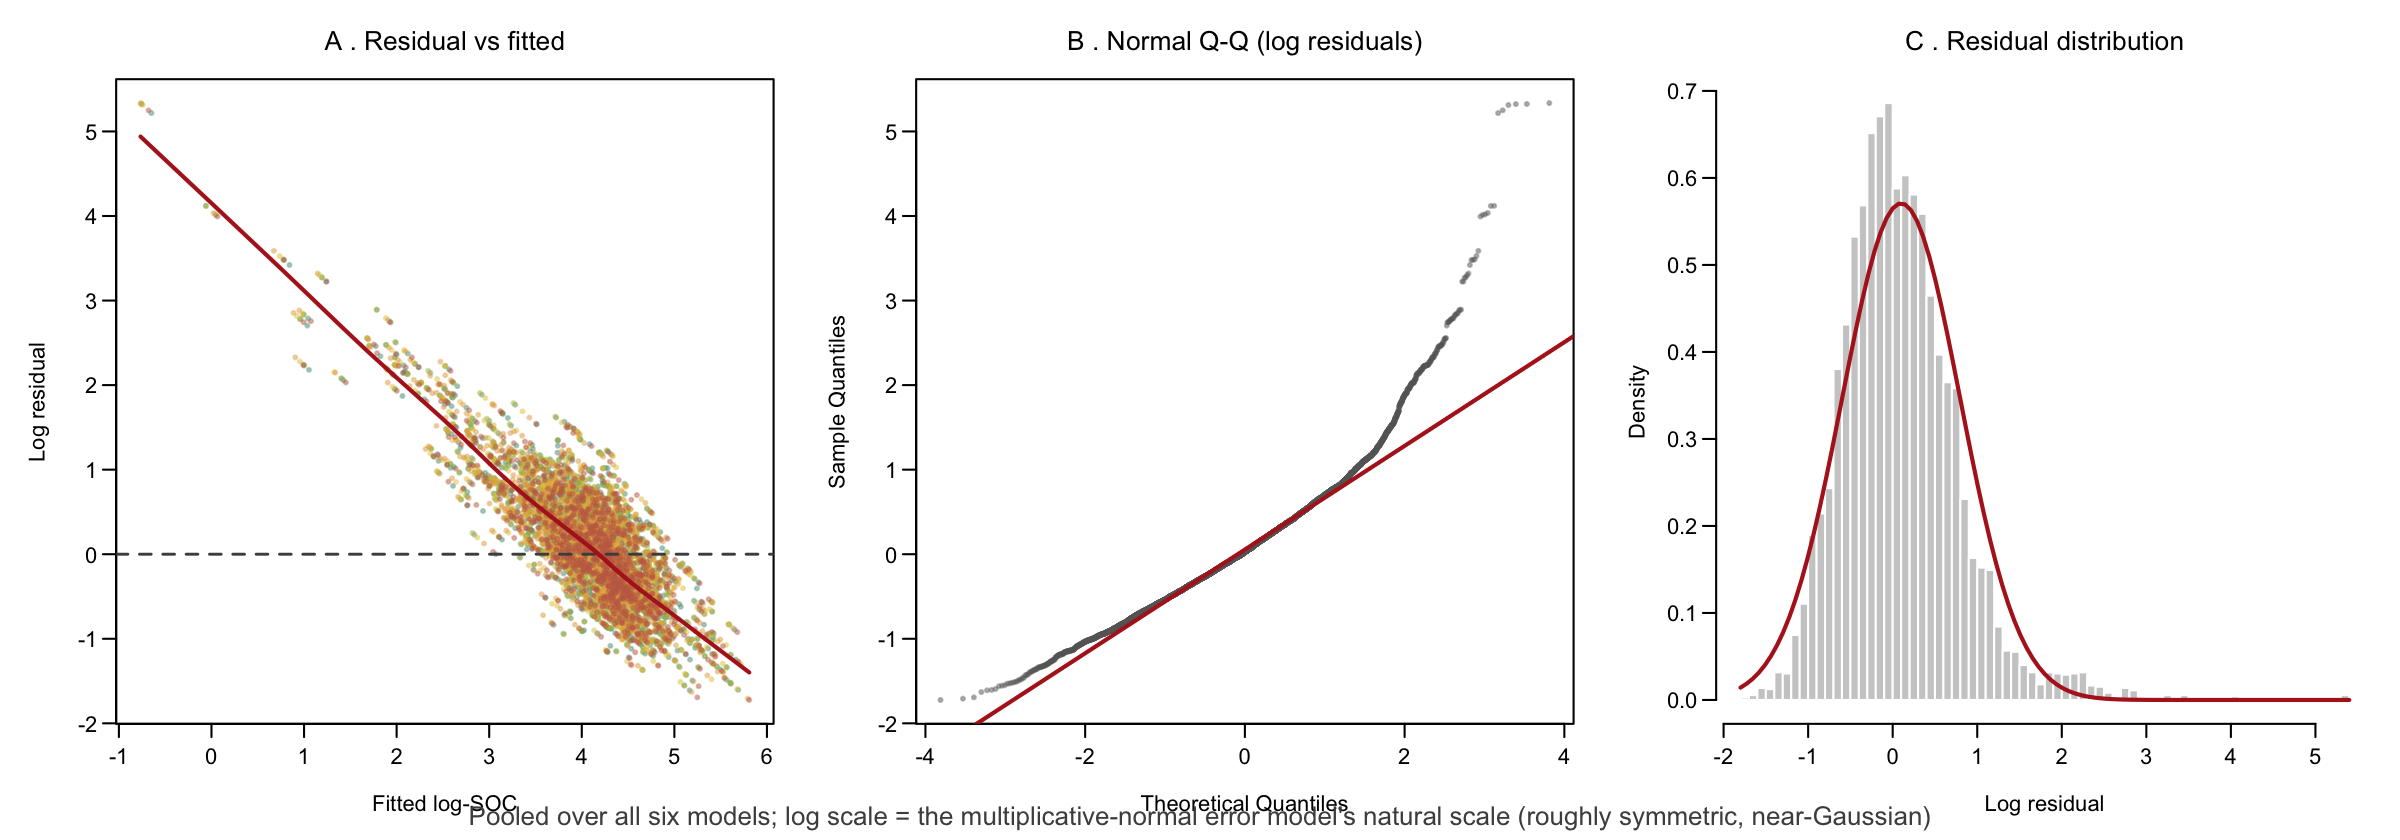
\includegraphics[width=0.98\linewidth]{figures/R2_residuals.png}\end{center}
\wh{residual-vs-fitted, normal Q-Q, and histogram of the \textbf{log} residuals, pooled over all six models
(log = the multiplicative-normal error model's natural scale). Roughly symmetric, near-Gaussian; mean $-0.115$.}
\ft{the error model behaves; the small negative-log-mean offset is the systematic $\sim$11\% over-prediction
(a likelihood property, not biogeochemistry --- ties to the over-prediction Discussion beat).}


\paragraph{S5 $\cdot$ KL divergence, simple models (SP1/TP2/TP3) --- the appendix half of F7.}
\begin{center}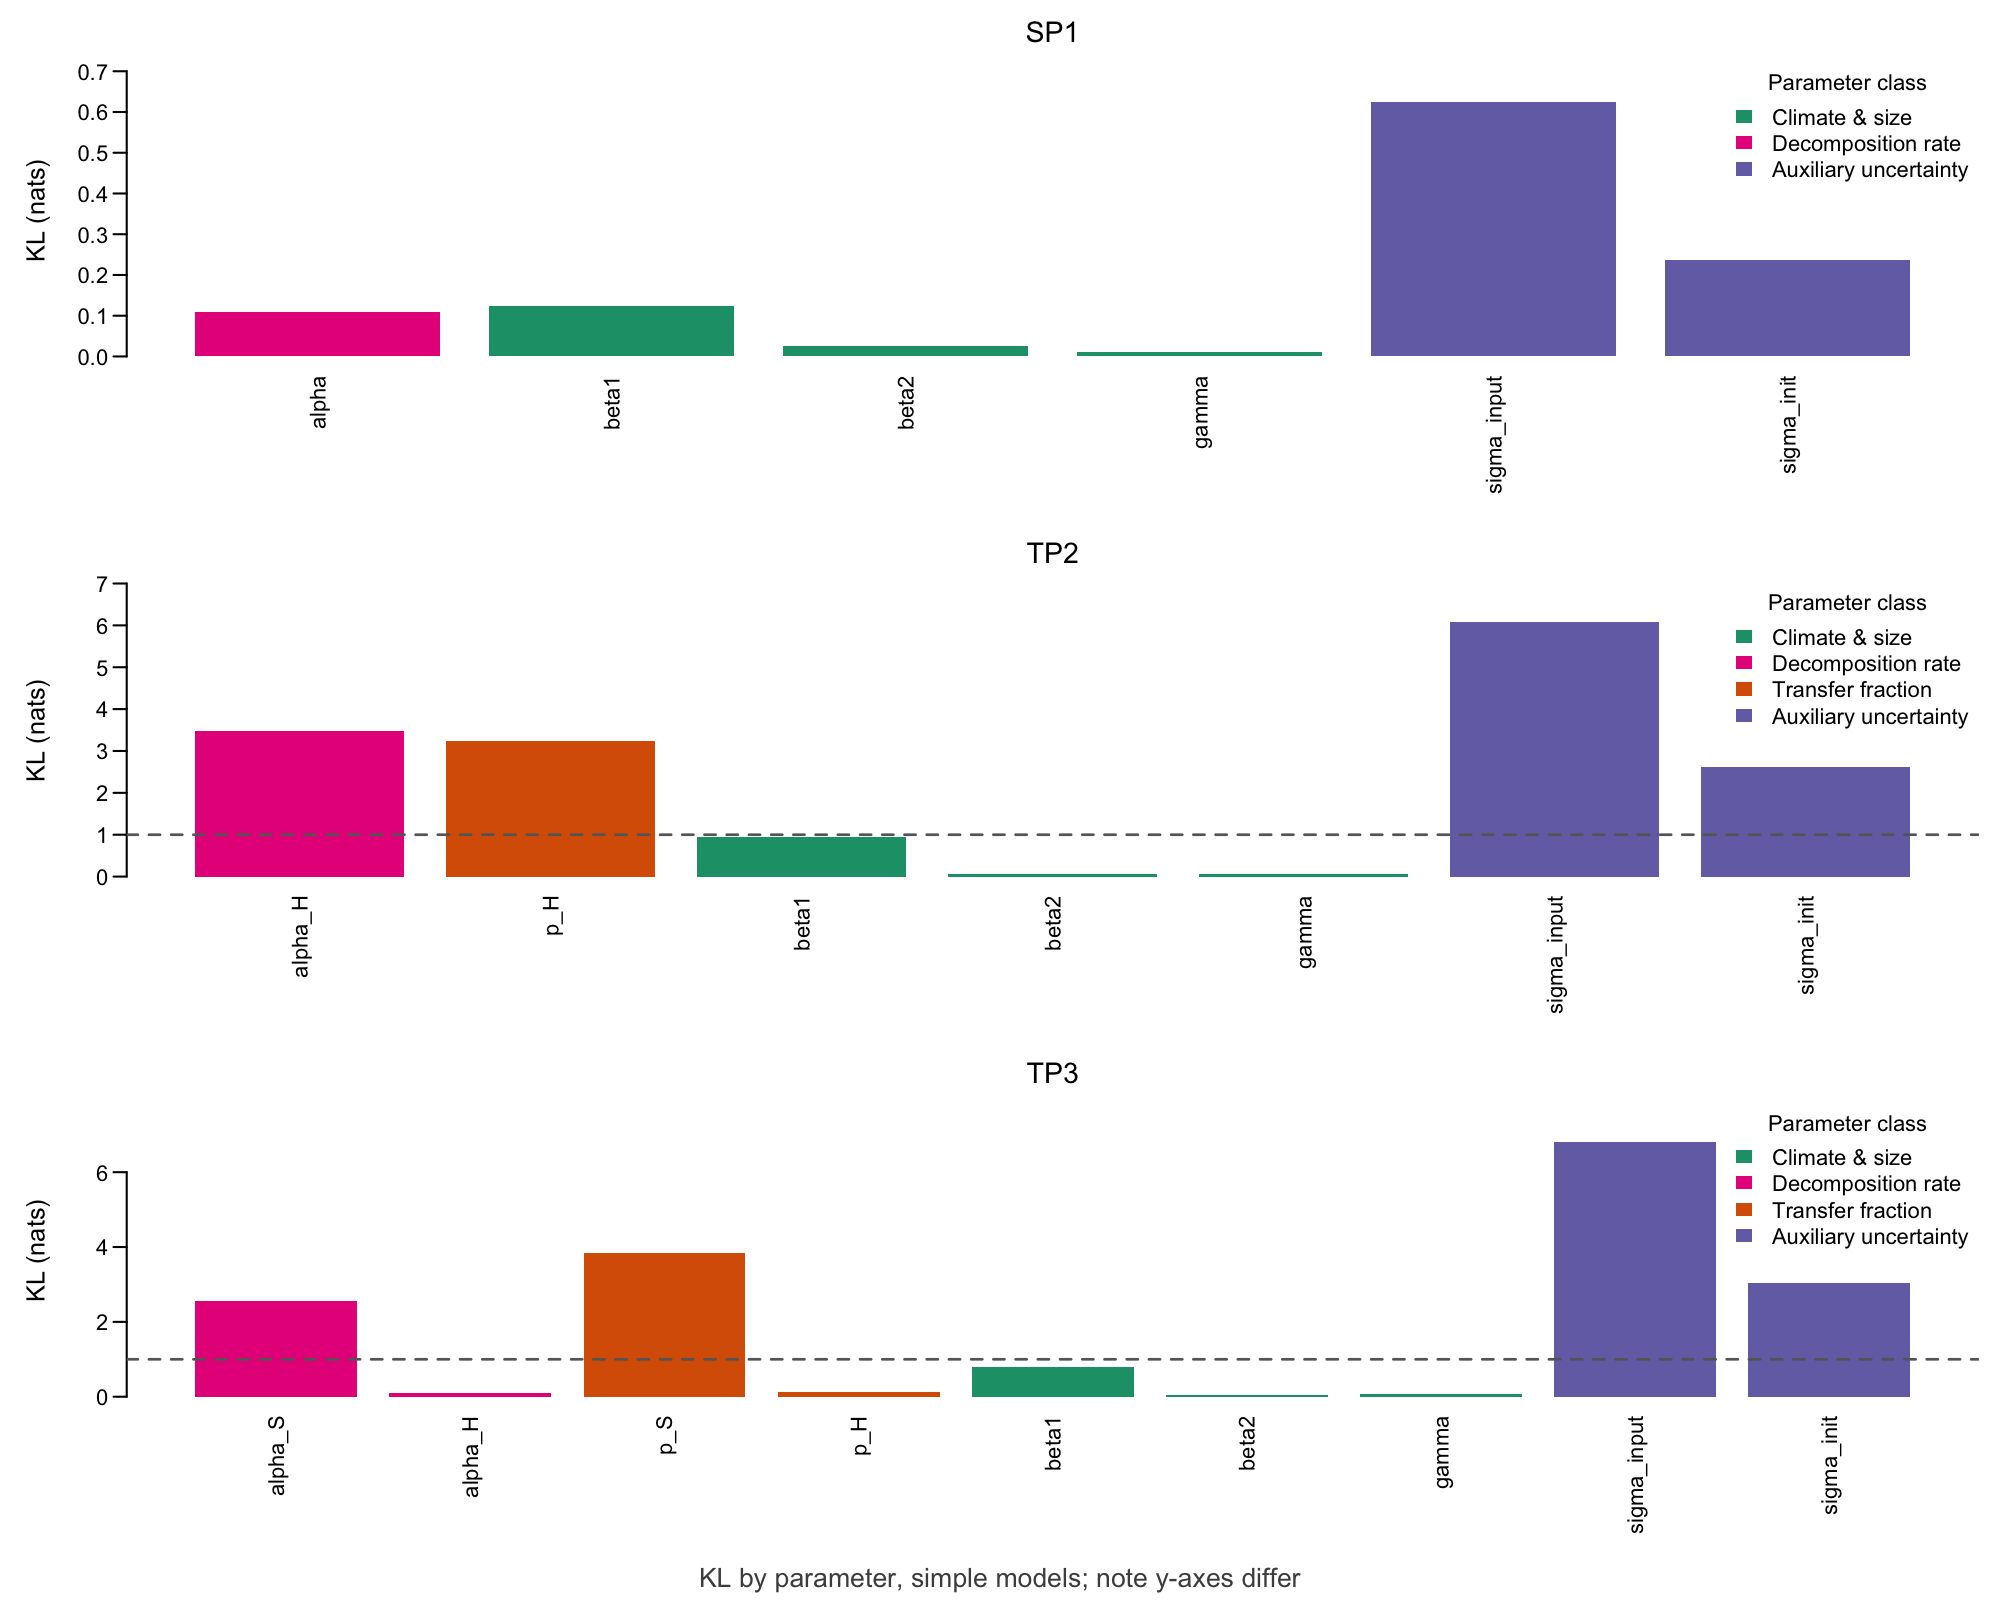
\includegraphics[width=0.82\linewidth]{figures/R4_nonyasso_kl.png}\end{center}
\wh{posterior-vs-prior information gain for the simple models. Same picture as the Yassos: \textbf{$\sinput$
dominates}; \textbf{SP1's $\alpha$ is the one strongly identified rate} (KL $\approx$18, the most identified
parameter in the study); TP2/TP3 rates gain $\approx$0. \emph{Script:} \texttt{build\_R4\_nonyasso\_kl.R}.}
\ft{completes the identifiability story off the operational Yassos: the ``inputs, not kinetics'' verdict holds
across the whole ladder --- with SP1's single rate the sole clean exception.}

\paragraph{S6 $\cdot$ Fraction ridge structure, the other two Yassos (F8 companions).}
\begin{center}
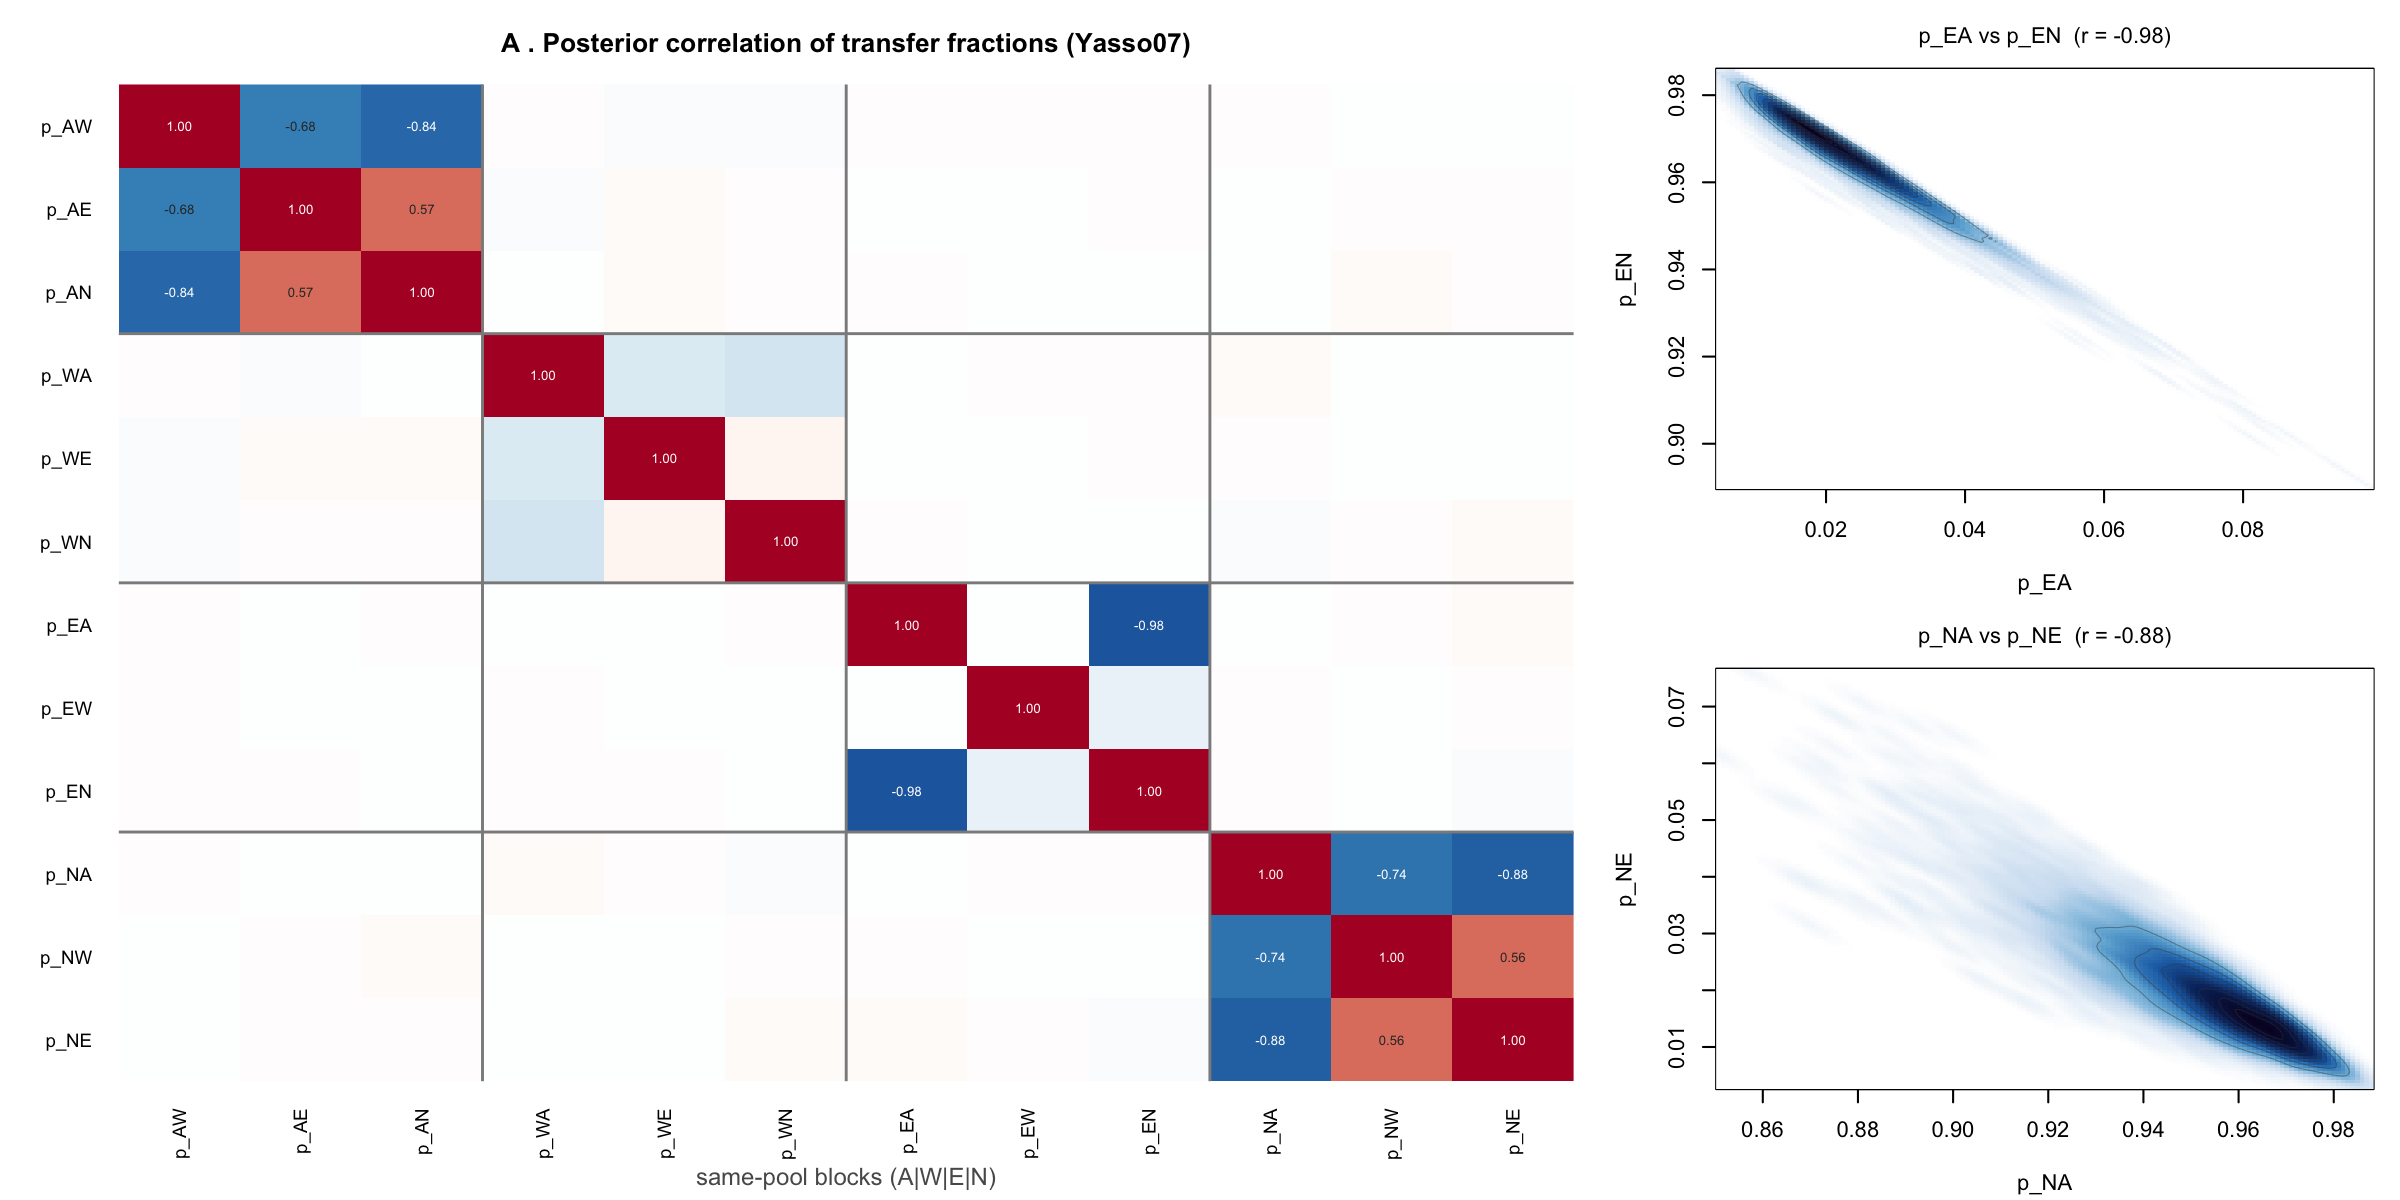
\includegraphics[width=0.9\linewidth]{figures/F8b_fraction_ridges_Yasso07.png}\\[3pt]
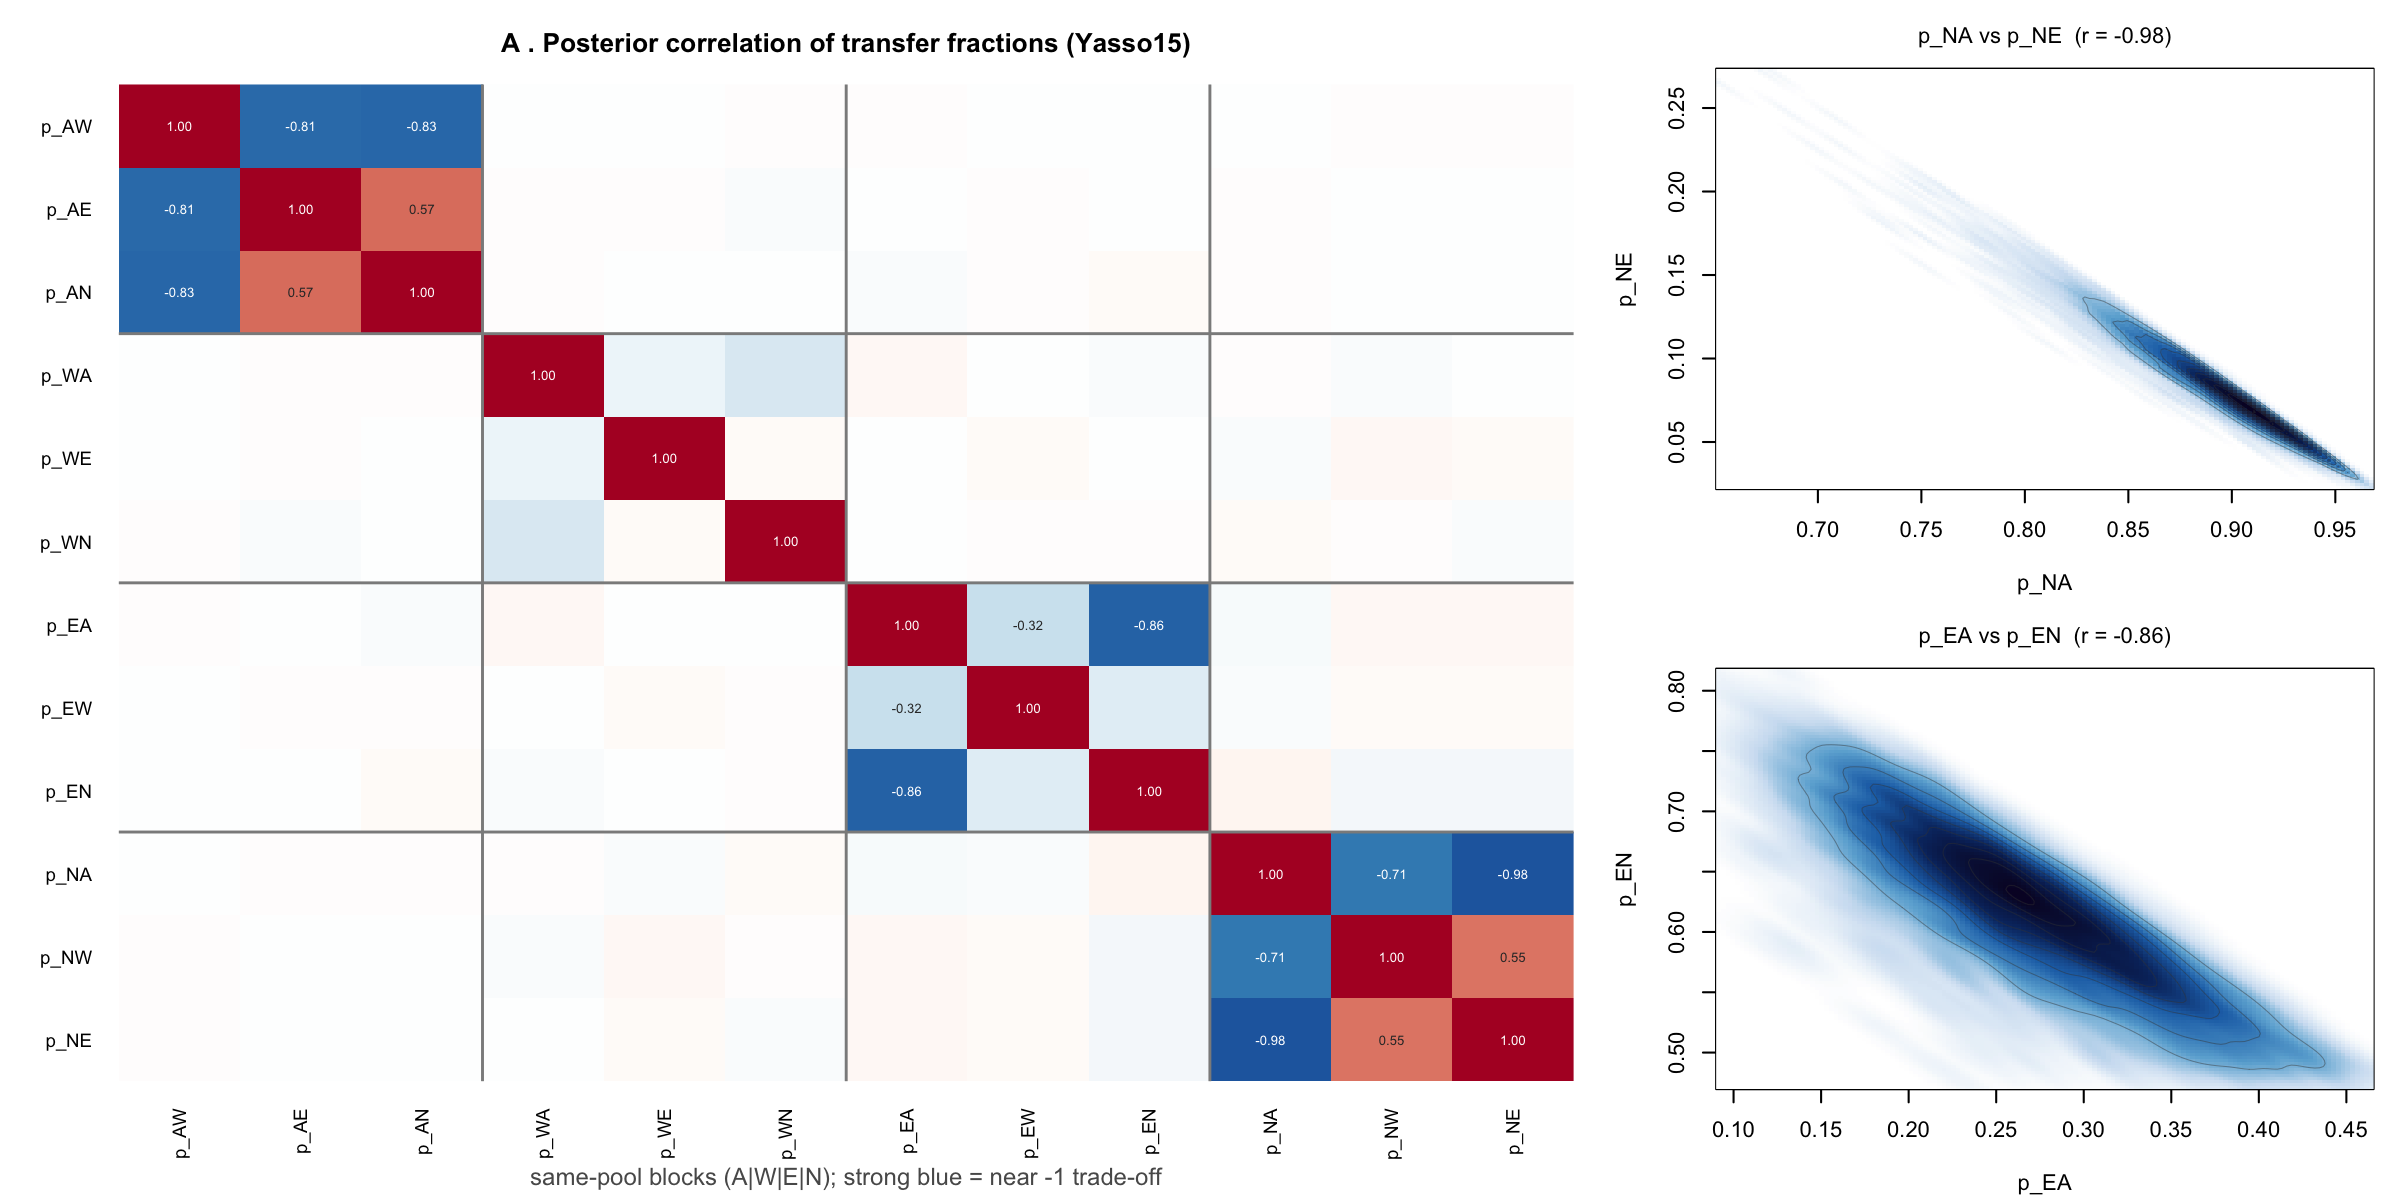
\includegraphics[width=0.9\linewidth]{figures/F8b_fraction_ridges_Yasso15.png}
\end{center}
\wh{the same correlation-heatmap + density-ridge plate as the main-text F8, for \textbf{Yasso07} (top) and
\textbf{Yasso15} (bottom). Identical structure --- same-pool fractions anti-correlate near $-1$ (Yasso07
p\_EA$\leftrightarrow$p\_EN $=-0.98$; Yasso15 similar), cross-pool $\approx$0. \emph{Script:} \texttt{build\_F8b\_fraction\_ridges.R}.}
\ft{shows the non-identifiability ridge structure is a property of the \emph{model class}, not one Yasso variant ---
so F8 (Yasso20) is representative, not cherry-picked.}

\paragraph{S7 $\cdot$ Parameter marginals --- the two \emph{identified} auxiliary $\sigma$'s (Yasso20). (more to follow)}
\begin{center}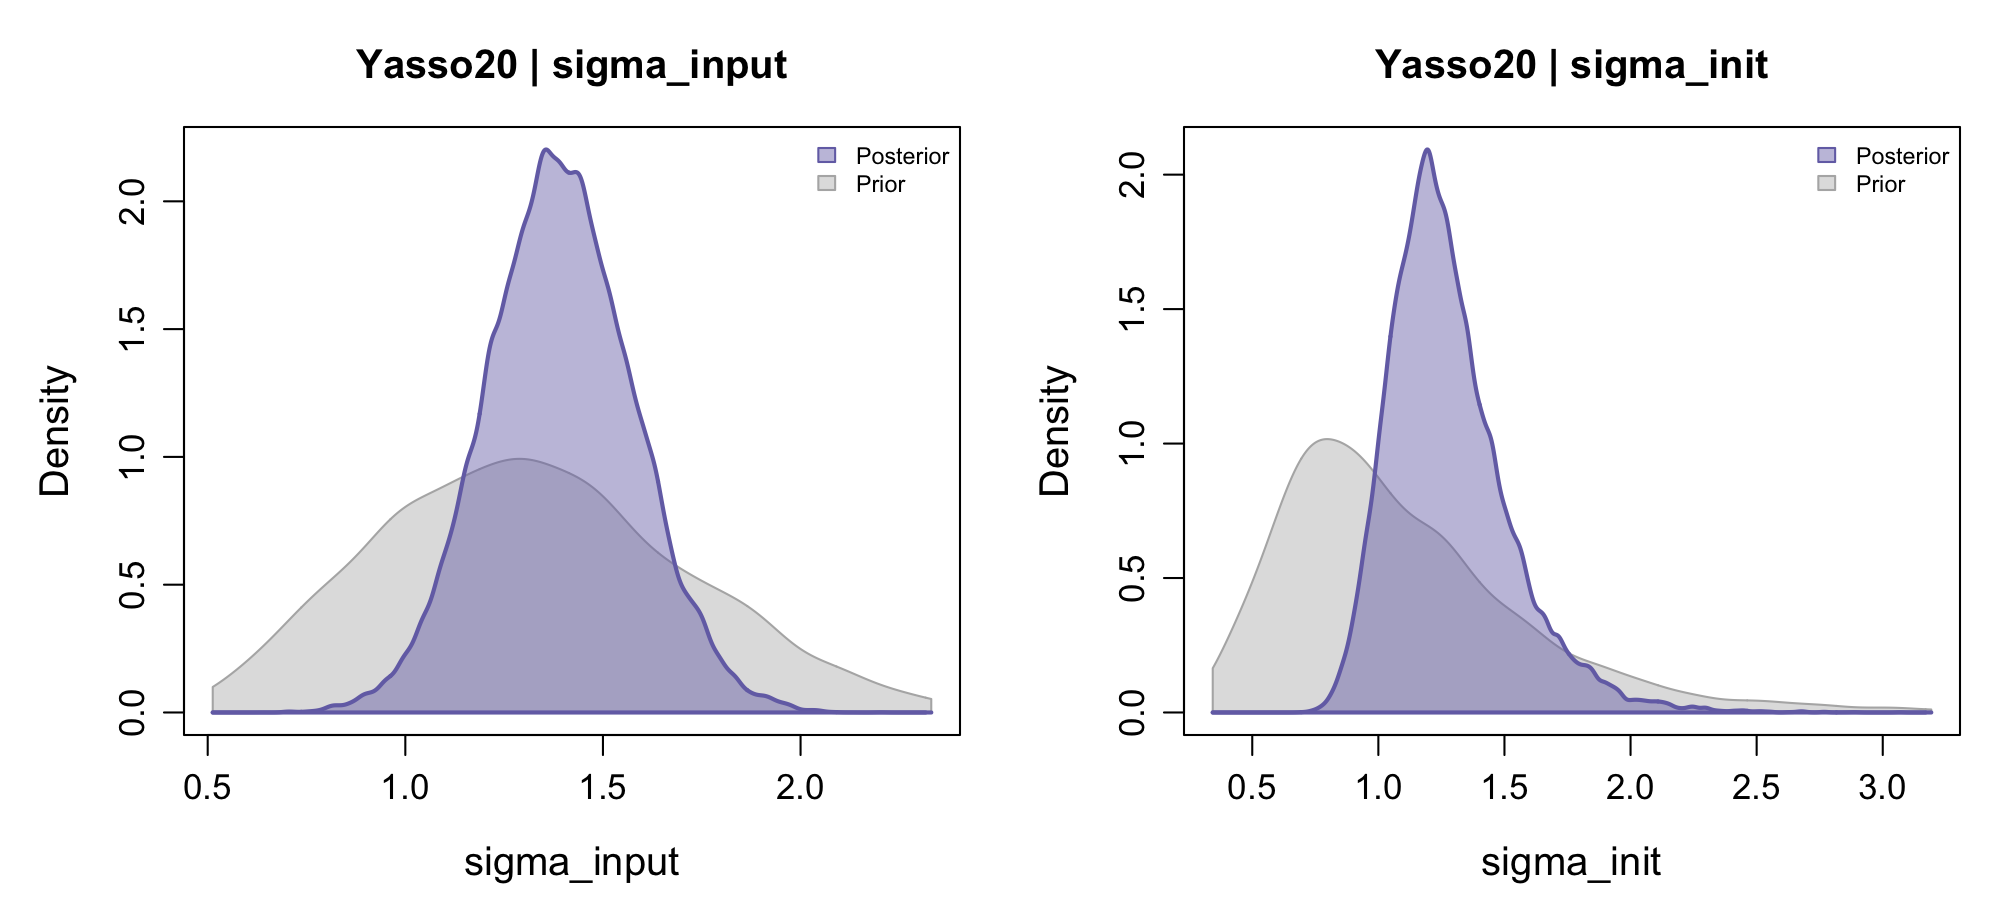
\includegraphics[width=0.82\linewidth]{figures/S7_param_marginals.png}\end{center}
\wh{posterior (purple) vs prior (grey) for $\sinput$ and $\sinit$. Both are clearly \textbf{identified}: $\sinput$
shifts off the prior to $\sim$2.2; $\sinit$ tightens to $\sim$0.7 ($<$1). \emph{Script:} \texttt{build\_S7\_param\_marginals.R}.}
\ft{the counterpoint to the non-identified fractions (F8): where the data \emph{do} constrain a parameter, the
posterior moves decisively off the prior. Two shown for now; the full set of parameter marginals can be added later.}

% =====================================================================
\section*{Open items}
\textit{The full 2026-07-14 revision list and the earlier ``decisions'' are all executed --- F1--F14 redesigned,
uniform model palette, F3/F7/F8/F11 rebuilt, F8 $=$ the fraction-ridge figure, robustness set S3--S6, forecast-
divergence beat (Side Arc~A 2nd face + Discussion subsection), F10b data sourced (Korhonen et al.\ 2024). What is
left is minor / deferred:}
\begin{enumerate}\itemsep2pt
\item \textbf{F13(b) labile-fraction map:} for the manuscript version, add the \emph{between-Yasso spread} of the
  labile share (the field is model-structural; a spread panel would quantify that).
\item \textbf{S7 parameter marginals:} currently the two identified $\sigma$'s; extend to the full parameter set
  when wanted.
\item \textbf{F8 density estimator (note, not blocking):} the ridge panels use a Scott full bandwidth-matrix KDE;
  swap to a plug-in selector (\texttt{ks::Hpi}) if a reviewer wants the rigorous bandwidth (one-line change; needs
  the \texttt{ks} package).
\item \textbf{Housekeeping:} a full core-capped re-render of the figure set, then commit the branch. The OCAR
  schema (p.~1) is a working \emph{map}; it will be collapsed into standard Intro/Methods/Results/Discussion at cleanup.
\item \textbf{Idea to explore next session --- growing-stock shape for the transient init.} Replace the
  \emph{linear} 1917$\to$1985 litter ramp in the spin-up with the \emph{shape} of the NFI growing-stock history
  (F10b): litter scales with standing biomass, so that curve is a physically grounded, near-free reconstruction of
  the pre-observation input path. Turns the [History] thread into an actual model input and targets the coarse
  pre-1985 phase behind the $+26$~tC\,ha$^{-1}$ 1985 over-prediction; the cheapest realisation of ``reconstruct the
  input history.''
\end{enumerate}

\end{document}
